% Nội dung chính thức của báo cáo LaTeX.
% Nội dung có thể tiếp tục chỉnh trực tiếp trong tệp này.

\chapter{GIỚI THIỆU VÀ PHÁT BIỂU BÀI TOÁN}
\label{ch:1}

\section{Bối cảnh}
\label{sec:1-1}

Hầu như mọi phần mềm có ô tìm kiếm đều phải giải quyết hai việc. Việc
thứ nhất là tìm mọi vị trí xuất hiện của một chuỗi trong một văn bản,
thứ mà người dùng gặp mỗi lần nhấn Ctrl+F trong trình soạn thảo, hoặc
mỗi lần một quản trị viên lọc log theo từ khóa. Việc thứ hai là đoán
phần còn lại của từ mà người dùng đang gõ dở, thứ xuất hiện ở thanh địa
chỉ trình duyệt, ở ô tìm kiếm của các trang thương mại điện tử, và ở
tính năng gợi ý mã lệnh của các IDE.

Nghe qua thì hai việc này giống nhau, vì cả hai đều được mô tả bằng cụm
từ ``tìm chuỗi''. Nhưng chúng khác nhau ở một điểm quyết định: cái gì
được biết trước khi truy vấn đến. Trong bài toán thứ nhất, cả văn bản
lẫn mẫu đều có thể là mới; ta không được phép giả định gì về chúng.
Trong bài toán thứ hai, từ điển gợi ý đã nằm sẵn trong bộ nhớ từ lúc
khởi động, chỉ có tiền tố truy vấn là mới. Sự khác biệt đó dẫn tới hai
chiến lược tiền xử lý trái ngược nhau, và từ đó là hai họ thuật toán
khác nhau.

\begin{center}
\captionof{table}{Đối chiếu hai bài toán và hệ quả về chiến lược tiền xử lý}
\end{center}

{\footnotesize\singlespacing
\begin{longtable}[]{@{}
  >{\raggedright\arraybackslash}p{(\linewidth - 4\tabcolsep) * \real{0.2526}}
  >{\raggedright\arraybackslash}p{(\linewidth - 4\tabcolsep) * \real{0.3595}}
  >{\raggedright\arraybackslash}p{(\linewidth - 4\tabcolsep) * \real{0.3596}}@{}}
\toprule\noalign{}
\begin{minipage}[b]{\linewidth}\raggedright
\end{minipage} & \begin{minipage}[b]{\linewidth}\raggedright
Tìm mẫu trong văn bản
\end{minipage} & \begin{minipage}[b]{\linewidth}\raggedright
Gợi ý theo tiền tố
\end{minipage} \\
\midrule\noalign{}
\endhead
\bottomrule\noalign{}
\endlastfoot
Cái gì biết trước & không gì cả & toàn bộ từ điển \\
Tiền xử lý phía nào & mẫu P & dữ liệu D \\
Thuật toán tương ứng & KMP & Trie \\
Chi phí một truy vấn & O(n + m) & O(\textbar q\textbar{} + V +
k·L\_max), với \textbar Σ′\textbar{} cố định \\
Phụ thuộc \textbar Σ\textbar{} & không & có \\
\end{longtable}
}

Bảng 1.1 là luận điểm trung tâm của báo cáo. Nó cũng giải thích vì sao
đề bài yêu cầu tách chuyên đề thành hai module độc lập thay vì trình bày
chúng như hai biến thể của một thuật toán duy nhất. Trong phần cài đặt,
tôi giữ ràng buộc này ở mức mã nguồn: hai gói src/kmp/ và src/trie/
không import lẫn nhau, và chỉ có tầng ứng dụng mới dùng cả hai.

Để hai module cùng chạy trên một luồng người dùng thật, tôi xây hệ thống
Interactive Text Search \& Autocomplete. Người dùng gõ vài ký tự đầu,
Trie trả về danh sách gợi ý; người dùng chọn một gợi ý, KMP tìm mọi vị
trí của nó trong văn bản và tô sáng kết quả. Hệ thống có hai giao diện,
một chạy trên dòng lệnh và một chạy trong trình duyệt.

\section{Module A --- So khớp mẫu tuyến tính bằng KMP}
\label{sec:1-2}

Đầu vào của module là văn bản T độ dài n và mẫu P độ dài m, cả hai trên
một alphabet Σ tùy ý. Đầu ra là tập mọi chỉ số i sao cho T{[}i..i+m−1{]}
trùng P, tính cả những lần xuất hiện overlapping. Chỉ số trả về theo quy
ước 0-based và tăng ngặt. Thuật toán KMP được Knuth, Morris và Pratt
trình bày trong công trình gốc về so khớp mẫu nhanh \cite{kmp1977}.

Điểm cần nhấn mạnh ngay từ phát biểu bài toán là KMP chỉ đòi hỏi phép so
sánh bằng giữa hai ký tự. Nó không cần một quan hệ thứ tự trên Σ, cũng
không cần Σ hữu hạn. Nhiều tài liệu trình bày KMP song song với
automaton hữu hạn, mà automaton thì cần \textbar Σ\textbar{} cột cho
bảng chuyển, nên dễ để lại ấn tượng sai rằng thuật toán phụ thuộc kích
thước alphabet. Phiên bản dùng prefix function thì không, và tôi kiểm
chứng điều này bằng cách chạy trực tiếp module trên chuỗi Unicode tiếng
Việt có dấu.

Về các trường hợp biên, tôi quy ước m = 0 bị từ chối tường minh bằng một
ngoại lệ chứ không trả về danh sách rỗng hay danh sách mọi vị trí. Lý do
là mẫu rỗng khớp ở mọi vị trí nên kết quả không mang thông tin, và việc
trả về {[}0..n{]} một cách im lặng sẽ trở thành cái bẫy cho tầng gọi.
Trường hợp m \textgreater{} n được xử lý bằng một nhánh riêng chứ không
dựa vào việc vòng lặp tự rỗng, vì tôi muốn ý định của mã nguồn hiện ra
rõ ràng khi đọc lại.

\begin{center}
\captionof{table}{Ví dụ minh họa cho module KMP}
\end{center}

{\footnotesize\singlespacing
\begin{longtable}[]{@{}
  >{\raggedright\arraybackslash}p{(\linewidth - 6\tabcolsep) * \real{0.2140}}
  >{\raggedright\arraybackslash}p{(\linewidth - 6\tabcolsep) * \real{0.2140}}
  >{\raggedright\arraybackslash}p{(\linewidth - 6\tabcolsep) * \real{0.2334}}
  >{\raggedright\arraybackslash}p{(\linewidth - 6\tabcolsep) * \real{0.3112}}@{}}
\toprule\noalign{}
\begin{minipage}[b]{\linewidth}\raggedright
T
\end{minipage} & \begin{minipage}[b]{\linewidth}\raggedright
P
\end{minipage} & \begin{minipage}[b]{\linewidth}\raggedright
Kết quả
\end{minipage} & \begin{minipage}[b]{\linewidth}\raggedright
Ghi chú
\end{minipage} \\
\midrule\noalign{}
\endhead
\bottomrule\noalign{}
\endlastfoot
aaaa & aa & {[}0, 1, 2{]} & ba lần, overlapping \\
mississippi & issi & {[}1, 4{]} & overlapping tại 1 và 4 \\
ababcabab & abab & {[}0, 5{]} & mẫu tuần hoàn \\
abc & abcd & {[}{]} & trường hợp m \textgreater{} n \\
a×1000 & a×999 + b & {[}{]} & trường hợp xấu nhất của naive \\
\end{longtable}
}

\section{Module B --- Lưu và truy vấn theo tiền tố bằng Trie}
\label{sec:1-3}

Đầu vào gồm từ điển D chứa N từ trên một alphabet Σ′ được khai báo rõ,
một tiền tố truy vấn q, và số kết quả tối đa k. Module phải hỗ trợ bốn
thao tác: insert để thêm từ, exact search trả về giá trị luận lý cho
biết một chuỗi có nằm trong D hay không, prefix query cho biết có từ nào
bắt đầu bằng q hay không, và autocomplete trả về nhiều nhất k từ mang
tiền tố q.

Phân biệt giữa exact search và prefix query là chỗ dễ nhầm. Với từ điển
chứa ``tin'' và ``tinh'', truy vấn exact search trên chuỗi ``ti'' phải
trả về sai, vì ``ti'' chỉ là tiền tố chứ không phải một từ; nhưng prefix
query trên cùng chuỗi đó lại phải trả về đúng. Trong cài đặt, hai thao
tác này khác nhau đúng một điều kiện: cùng đi xuống theo chuỗi truy vấn,
nhưng exact search còn phải kiểm tra cờ đánh dấu cuối từ tại nút đích.

Về xử lý ký tự nằm ngoài alphabet, tôi chọn hai hành vi khác nhau cho
hai nhóm thao tác, và sự khác biệt này là có chủ ý. Khi insert gặp ký tự
lạ, module ném ngoại lệ kèm theo chính ký tự vi phạm và vị trí của nó
trong chuỗi. Khi truy vấn gặp ký tự lạ, module trả về kết quả rỗng chứ
không ném lỗi. Lý do là hỏi về một từ không thể tồn tại vẫn là một câu
hỏi hợp lệ, còn đưa vào từ điển một từ sai alphabet thì là lỗi dữ liệu
và cần được phát hiện sớm.

\begin{center}
\captionof{table}{Ví dụ minh họa cho module Trie, với D = \{tin, tinh, to, toan, a, an, and, ant, banana\}}
\end{center}

{\footnotesize\singlespacing
\begin{longtable}[]{@{}
  >{\raggedright\arraybackslash}p{(\linewidth - 4\tabcolsep) * \real{0.2915}}
  >{\raggedright\arraybackslash}p{(\linewidth - 4\tabcolsep) * \real{0.3886}}
  >{\raggedright\arraybackslash}p{(\linewidth - 4\tabcolsep) * \real{0.2916}}@{}}
\toprule\noalign{}
\begin{minipage}[b]{\linewidth}\raggedright
Truy vấn
\end{minipage} & \begin{minipage}[b]{\linewidth}\raggedright
Kết quả
\end{minipage} & \begin{minipage}[b]{\linewidth}\raggedright
Ghi chú
\end{minipage} \\
\midrule\noalign{}
\endhead
\bottomrule\noalign{}
\endlastfoot
search("tin") & True & là một từ trong D \\
search("ti") & False & chỉ là tiền tố \\
starts\_with("ti") & True & ngược lại với dòng trên \\
autocomplete("t", 10) & {[}tin, tinh, to, toan{]} & truncated = False \\
autocomplete("t", 2) & {[}tin, tinh{]} & truncated = True \\
autocomplete("", 3) & {[}a, an, and{]} & tiền tố rỗng \\
\end{longtable}
}

Thứ tự kết quả trả về là thứ tự từ điển theo code point, và tính xác
định này không phải chi tiết thẩm mỹ. Nếu thứ tự không xác định thì việc
đối chiếu tự động với baseline sẽ không thực hiện được, và toàn bộ chiến
lược kiểm thử ở Chương 6 sẽ mất chỗ dựa.

\section{Kiến trúc hệ thống}
\label{sec:1-4}

\begin{quote}
người dùng gõ người dùng chọn gợi ý

\textbar{} \textbar{}

v v

+-\/-\/-\/-\/-\/-\/-\/-\/-\/-\/-\/-\/-\/-\/-\/-\/-+
+-\/-\/-\/-\/-\/-\/-\/-\/-\/-\/-\/-\/-\/-\/-\/-\/-+

\textbar{} MODULE B \textbar{} gợi ý (\textless= k từ) \textbar{} MODULE
A \textbar{}

\textbar{} Trie
\textbar-\/-\/-\/-\/-\/-\/-\/-\/-\/-\/-\/-\/-\/-\/-\/-\/-\/-\/-\/-\/-\textgreater\textbar{}
KMP \textbar{}

\textbar{} autocomplete \textbar{} \textbar{} kmp\_search \textbar{}

+-\/-\/-\/-\/-\/-\/-\/-\/-\/-\/-\/-\/-\/-\/-\/-\/-+
+-\/-\/-\/-\/-\/-\/-\/-\/-\/-\/-\/-\/-\/-\/-\/-\/-+

\textbar{} \textbar{}

O(\textbar q\textbar{} + V + k*L\_max) O(n + m)

\textbar{} \textbar{}

v v

danh sách gợi ý vị trí khớp + tô sáng
\end{quote}

\begin{center}
\captionof{figure}{Kiến trúc hệ thống Interactive Text Search \& Autocomplete. Hai module độc lập, chỉ gặp nhau ở tầng ứng dụng}
\end{center}

\section{Mục tiêu và phạm vi của chuyên đề}
\label{sec:1-5}

\begin{enumerate}
\def\labelenumi{\arabic{enumi}.}
\item
  Cài đặt hai module đạt đúng độ phức tạp lý thuyết, có xử lý đầy đủ các
  trường hợp biên và dữ liệu không hợp lệ.
\item
  Chứng minh tính đúng đắn bằng lập luận toán học, không dừng ở mức mô
  tả mã nguồn.
\item
  Kiểm chứng phân tích độ phức tạp bằng số liệu thực nghiệm, đối chiếu
  với baseline độc lập.
\item
  Mô hình hóa một ứng dụng thực tế và nêu trung thực những gì hệ thống
  làm không tốt.
\end{enumerate}

Phạm vi báo cáo không bao gồm các cấu trúc chỉ mục dựa trên hậu tố như
suffix tree \cite{ukkonen1995} hay suffix array \cite{manber1993}, dù chúng là lựa chọn
đúng khi cần truy vấn nhiều lần trên một văn bản cố định. Lý do được
trình bày ở Mục 7.3.

\chapter{CƠ SỞ LÝ THUYẾT}
\label{ch:2}

\section{Ký hiệu và định nghĩa}
\label{sec:2-1}

Phần này định nghĩa mọi ký hiệu sẽ dùng về sau. Cách trình bày bám theo
quy ước trong \cite{cormen2022,gusfield1997}.

Cho chuỗi S độ dài \textbar S\textbar{} = k trên alphabet Σ. Ký hiệu
S{[}i..j{]} là chuỗi con liên tiếp từ chỉ số i đến j, bao gồm cả hai
đầu. Một tiền tố của S là chuỗi S{[}0..i{]} với 0 ≤ i \textless{} k;
tiền tố đó gọi là thật sự nếu i \textless{} k−1, tức là nó khác chính S.
Định nghĩa đối ngẫu cho hậu tố.

\begin{quote}
\textbf{Định nghĩa 2.1 (border).} Chuỗi B gọi là \emph{border} của chuỗi
S nếu B vừa là tiền tố thật sự vừa là hậu tố thật sự của S. Chuỗi rỗng
luôn là border của mọi chuỗi khác rỗng.
\end{quote}

Thuật ngữ border được giữ nguyên tiếng Anh trong toàn bộ báo cáo. Cách
dịch thường gặp là ``biên'', nhưng từ này đã mang nghĩa khác trong ngữ
cảnh kiểm thử biên nên dễ gây nhầm.

Về ký hiệu kích thước bài toán, tôi dùng n cho độ dài văn bản, m cho độ
dài mẫu, N cho số từ trong từ điển, L cho độ dài một từ và L\_max cho độ
dài từ dài nhất. Điều quan trọng cần nói rõ ngay là biến nào thực sự
quyết định chi phí. Với module A, đó là n và m; \textbar Σ\textbar{}
không xuất hiện trong bất kỳ chặn nào. Với module B, chi phí một thao
tác chỉ phụ thuộc L, còn N và \textbar Σ′\textbar{} chỉ ảnh hưởng tới bộ
nhớ.

\section{Prefix function}
\label{sec:2-2}

\begin{quote}
\textbf{Định nghĩa 2.2 (prefix function).} Với mẫu P độ dài m, hàm π:
\{0,\ldots,m−1\} → \{0,\ldots,m−1\} xác định bởi π{[}i{]} = độ dài
border dài nhất của P{[}0..i{]}.
\end{quote}

Trong tài liệu tiếng Anh, mảng này thường được gọi là LPS, viết tắt của
longest proper prefix which is also suffix. Tôi dùng cả hai cách gọi, π
khi nói về hàm toán học và LPS khi nói về mảng trong mã nguồn.

\begin{center}
\captionof{table}{Giá trị π của mẫu P = "ababaca"}
\end{center}

{\footnotesize\singlespacing
\begin{longtable}[]{@{}
  >{\raggedright\arraybackslash}p{(\linewidth - 14\tabcolsep) * \real{0.1563}}
  >{\centering\arraybackslash}p{(\linewidth - 14\tabcolsep) * \real{0.1173}}
  >{\centering\arraybackslash}p{(\linewidth - 14\tabcolsep) * \real{0.1173}}
  >{\centering\arraybackslash}p{(\linewidth - 14\tabcolsep) * \real{0.1173}}
  >{\centering\arraybackslash}p{(\linewidth - 14\tabcolsep) * \real{0.1173}}
  >{\centering\arraybackslash}p{(\linewidth - 14\tabcolsep) * \real{0.1173}}
  >{\centering\arraybackslash}p{(\linewidth - 14\tabcolsep) * \real{0.1173}}
  >{\centering\arraybackslash}p{(\linewidth - 14\tabcolsep) * \real{0.1170}}@{}}
\toprule\noalign{}
\begin{minipage}[b]{\linewidth}\raggedright
i
\end{minipage} & \begin{minipage}[b]{\linewidth}\centering
0
\end{minipage} & \begin{minipage}[b]{\linewidth}\centering
1
\end{minipage} & \begin{minipage}[b]{\linewidth}\centering
2
\end{minipage} & \begin{minipage}[b]{\linewidth}\centering
3
\end{minipage} & \begin{minipage}[b]{\linewidth}\centering
4
\end{minipage} & \begin{minipage}[b]{\linewidth}\centering
5
\end{minipage} & \begin{minipage}[b]{\linewidth}\centering
6
\end{minipage} \\
\midrule\noalign{}
\endhead
\bottomrule\noalign{}
\endlastfoot
P{[}i{]} & a & b & a & b & a & c & a \\
π{[}i{]} & 0 & 0 & 1 & 2 & 3 & 0 & 1 \\
\end{longtable}
}

Lấy ví dụ giá trị π{[}4{]} = 3. Chuỗi P{[}0..4{]} là "ababa", các border
của nó gồm "aba" độ dài 3 và "a" độ dài 1; border dài nhất có độ dài 3,
đúng như bảng ghi.

\begin{quote}
\textbf{Bổ đề 2.3 (chuỗi border).} Tập độ dài của \emph{mọi} border của
chuỗi S độ dài k chính là dãy π{[}k−1{]}, π{[}π{[}k−1{]}−1{]},
π{[}π{[}π{[}k−1{]}−1{]}−1{]}, \ldots, 0.
\end{quote}

\emph{Chứng minh.} Trước hết, nếu B là border của S và B′ là border của
B thì B′ là tiền tố của B nên là tiền tố của S, đồng thời là hậu tố của
B nên là hậu tố của S; vậy B′ cũng là border của S. Chiều ngược lại, xét
một border C của S có độ dài nhỏ hơn border dài nhất B. Vì cả C và B đều
là tiền tố của S và \textbar C\textbar{} \textless{}
\textbar B\textbar{} nên C là tiền tố của B; lập luận đối ngẫu cho hậu
tố. Do đó C là border của B. Kết hợp hai chiều, tập border của S bằng
hợp của border dài nhất với tập border của chính border dài nhất đó, và
truy hồi này sinh đúng dãy đã nêu \(\blacksquare\)

Bổ đề 2.3 là nền tảng của toàn bộ Chương 3. Nội dung thực tế của nó là:
khi một border độ dài L không dùng được nữa, border dài nhất tiếp theo
có độ dài đúng bằng π{[}L−1{]}. Nói cách khác, ta có một cách nhảy trực
tiếp tới ứng viên tiếp theo mà không phải thử tuần tự.

Áp dụng vào P = "abaaba" với π = {[}0,0,1,1,2,3{]}, dãy border của toàn
mẫu là 3 → π{[}2{]} = 1 → π{[}0{]} = 0, ứng với ba chuỗi "aba", "a" và
chuỗi rỗng. Trong cài đặt, phương thức borders() của lớp KMPMatcher trả
về đúng dãy này và được dùng để minh họa trực quan khi trình bày.

\begin{quote}
\textbf{Bổ đề 2.4 (tăng chậm).} Với mọi i ≥ 1 ta có π{[}i{]} ≤
π{[}i−1{]} + 1.
\end{quote}

\emph{Chứng minh.} Giả sử π{[}i{]} = L \textgreater{} 0. Khi đó
P{[}0..L−1{]} là hậu tố của P{[}0..i{]}, nên bỏ ký tự cuối của cả hai vế
ta được P{[}0..L−2{]} là hậu tố của P{[}0..i−1{]}; đồng thời
P{[}0..L−2{]} hiển nhiên là tiền tố thật sự của P{[}0..i−1{]}. Vậy
P{[}0..L−2{]} là một border của P{[}0..i−1{]}, suy ra L−1 ≤ π{[}i−1{]} \(\blacksquare\)

Bổ đề này nhỏ nhưng là điều kiện then chốt để amortized analysis ở Mục
4.1 hoạt động: nó bảo đảm biến trạng thái của thuật toán chỉ tăng tối đa
một đơn vị mỗi bước, trong khi có thể giảm nhiều đơn vị. Chính sự bất
đối xứng đó cho phép ta dùng lập luận về hàm thế.

\section{Bất biến của KMP}
\label{sec:2-3}

Toàn bộ trạng thái mà KMP mang theo giữa các bước là một số nguyên duy
nhất, ký hiệu i. Bất biến của vòng lặp chính, mà tôi sẽ gọi là (BB-A)
trong suốt báo cáo, phát biểu như sau.

\begin{quote}
\textbf{Bất biến (BB-A).} Trước khi xử lý ký tự T{[}j{]}, giá trị i là
độ dài lớn nhất nhỏ hơn m sao cho P{[}0..i−1{]} là hậu tố của
T{[}0..j−1{]}. Ràng buộc i \textless{} m loại trạng thái chấp nhận đã
được báo ở bước trước.
\end{quote}

Điểm tinh tế nằm ở chỗ trạng thái này là một số nguyên chứ không phải
một tập vị trí. Thuật toán naive ngầm mang theo tập các vị trí bắt đầu
còn khả dĩ và phải kiểm tra lại từng vị trí; KMP nén toàn bộ thông tin
đó vào một con số, và đó chính là lý do con trỏ văn bản không bao giờ
phải lùi.

\section{Bất biến của Trie}
\label{sec:2-4}

Trie là cây có gốc, mỗi cạnh mang nhãn là một ký tự thuộc Σ′. Cấu trúc
này được Fredkin đề xuất từ năm 1960 \cite{fredkin1960} và tên gọi của nó lấy từ
giữa chữ retrieval. Ký hiệu str(u) là chuỗi ghép các nhãn dọc đường đi
từ gốc tới nút u. Cài đặt của tôi duy trì bốn bất biến sau.

\begin{itemize}
\item
  \textbf{(I1)} Mỗi nút u biểu diễn đúng một tiền tố, là str(u). Gốc
  biểu diễn tiền tố rỗng.
\item
  \textbf{(I2)} Cờ is\_end tại u bằng đúng khi và chỉ khi str(u) là một
  từ thuộc D.
\item
  \textbf{(I3)} Trường word\_count tại u đếm số lần str(u) đã được
  insert; is\_end tương đương word\_count \textgreater{} 0.
\item
  \textbf{(I4)} Trường prefix\_count tại u bằng tổng word\_count trên
  toàn bộ cây con gốc u, tức số lần insert của mọi từ mang tiền tố
  str(u).
\end{itemize}

Bất biến I1 kéo theo tính chất quan trọng nhất của Trie: hai từ có tiền
tố chung dùng chung đường đi, nên bộ nhớ tỉ lệ với số tiền tố phân biệt
chứ không phải tổng độ dài các từ. Thí nghiệm E3 ở Mục 6.6 đo trực tiếp
tỉ số này và cho thấy nó giảm dần khi từ điển lớn lên.

Bất biến I4 ít gặp trong các cài đặt Trie giáo khoa nhưng rất tiện. Nhờ
nó, câu hỏi ``có bao nhiêu từ mang tiền tố q'' được trả lời trong
O(\textbar q\textbar) thay vì phải duyệt toàn bộ cây con. Trong giao
diện web, con số hiển thị dạng ``8 trên 2 513 kết quả'' lấy trực tiếp từ
trường này.

\section{Phân biệt điều kiện bắt buộc và điều kiện đủ}
\label{sec:2-5}

Một trong những lỗi bị trừ điểm nặng theo yêu cầu của chuyên đề là nhầm
lẫn điều kiện áp dụng. Bảng 2.2 tách bạch những điều kiện thực sự bắt
buộc, tức là nếu vi phạm thì thuật toán sai hoặc không định nghĩa được,
khỏi những điều kiện chỉ là đủ, tức là làm mọi thứ tiện hơn nhưng vi
phạm thì hệ thống vẫn đúng.

\begin{center}
\captionof{table}{Phân biệt điều kiện bắt buộc và điều kiện đủ}
\end{center}

{\footnotesize\singlespacing
\begin{longtable}[]{@{}
  >{\raggedright\arraybackslash}p{(\linewidth - 4\tabcolsep) * \real{0.3303}}
  >{\raggedright\arraybackslash}p{(\linewidth - 4\tabcolsep) * \real{0.2138}}
  >{\raggedright\arraybackslash}p{(\linewidth - 4\tabcolsep) * \real{0.4275}}@{}}
\toprule\noalign{}
\begin{minipage}[b]{\linewidth}\raggedright
Điều kiện
\end{minipage} & \begin{minipage}[b]{\linewidth}\raggedright
Loại
\end{minipage} & \begin{minipage}[b]{\linewidth}\raggedright
Hệ quả nếu vi phạm
\end{minipage} \\
\midrule\noalign{}
\endhead
\bottomrule\noalign{}
\endlastfoot
Ký tự so sánh được bằng phép bằng & bắt buộc (KMP) & thuật toán không
định nghĩa được \\
So sánh hai ký tự tốn O(1) & bắt buộc cho chặn O(n+m) & độ phức tạp nhân
thêm chi phí so sánh \\
Σ hữu hạn & không cần cho KMP & KMP vẫn đúng và vẫn tuyến tính \\
Σ′ hữu hạn, khai báo trước & bắt buộc (Trie) & không chọn được cách lưu
cạnh, không kiểm tra được đầu vào \\
Từ điển đã chuẩn hóa NFC & đủ & vẫn đúng, nhưng các dạng hiển thị giống
nhau tách thành nhánh khác nhau \\
Văn bản vừa trong RAM & đủ & cần phiên bản streaming; (BB-A) vẫn giữ
nguyên \\
Không xóa khỏi Trie & đủ & cần thêm thao tác delete bảo toàn I3 và I4 \\
\end{longtable}
}

Dòng thứ ba trong bảng đáng được nói thêm. Nhiều tài liệu trình bày KMP
cùng với string matching automaton, mà automaton cần bảng chuyển kích
thước m × \textbar Σ\textbar, nên người đọc dễ kết luận rằng KMP phụ
thuộc alphabet. Phiên bản dùng prefix function thì không, và tôi kiểm
chứng bằng một test chạy trên chuỗi tiếng Việt có dấu, nơi mỗi ký tự là
một code point Unicode chứ không phải một byte.

\chapter{THUẬT TOÁN VÀ CHỨNG MINH\\TÍNH ĐÚNG ĐẮN}
\label{ch:3}

Chương này trình bày mã giả của cả hai module rồi chứng minh chúng đúng.
Cách tổ chức bám theo lối trình bày của Cormen và cộng sự \cite{cormen2022}: phát
biểu bất biến trước, chứng minh bất biến được bảo toàn, rồi rút ra tính
đúng đắn của thuật toán như hệ quả.

\section{Xây dựng prefix function}
\label{sec:3-1}

\begin{quote}
BUILD\_LPS(P): \# P{[}0..m-1{]}

1 pi{[}0{]} \textless- 0

2 length \textless- 0 \# bất biến: length = pi{[}i-1{]}

3 for i \textless- 1 to m-1:

4 loop:

5 if P{[}i{]} = P{[}length{]}: \# thử mở rộng border hiện tại

6 length \textless- length + 1

7 break

8 if length = 0: \# không còn border để lùi

9 break

10 length \textless- pi{[}length-1{]} \# lùi theo Bổ đề 2.3

11 pi{[}i{]} \textless- length

12 return pi
\end{quote}

\begin{center}
\textbf{Thuật toán.} Xây dựng prefix function trong thời gian tuyến tính.
\end{center}

Ý tưởng của vòng lặp là như sau. Ở bước i, ta đã biết length bằng
π{[}i−1{]}, tức độ dài border dài nhất của P{[}0..i−1{]}. Mọi border của
P{[}0..i{]} đều phải có dạng một border B của P{[}0..i−1{]} nối thêm ký
tự P{[}i{]}, với điều kiện ký tự đứng ngay sau B trong mẫu, tức
P{[}\textbar B\textbar{]}, bằng đúng P{[}i{]}. Vòng loop ở dòng 4 thử
lần lượt các border B theo thứ tự độ dài giảm dần, đúng dãy mà Bổ đề 2.3
mô tả. Do dãy giảm, border hợp lệ đầu tiên tìm được cũng là border dài
nhất.

\begin{quote}
\textbf{Định lý 3.1.} Thuật toán BUILD\_LPS trả về đúng hàm π theo Định
nghĩa 2.2.
\end{quote}

\emph{Chứng minh.} Ta quy nạp theo \(i\). Với \(i=0\), chuỗi
\(P[0..0]\) chỉ có một ký tự nên border thật sự duy nhất là chuỗi rỗng;
dòng 1 đặt \(\pi[0]=0\). Giả sử \(\pi[0..i-1]\) đã đúng và khi vào bước
\(i\) ta có \(\mathit{length}=\pi[i-1]\).

Đặt \(L\) là giá trị đúng của \(\pi[i]\). Nếu \(L>0\), bỏ ký tự cuối của
border \(P[0..L-1]\) cho ta border độ dài \(L-1\) của \(P[0..i-1]\).
Theo Bổ đề 2.3, vòng lặp sẽ xét độ dài này; điều kiện
\(P[L-1]=P[i]\) cho phép mở rộng nó thành border độ dài \(L\).
Vì các độ dài ứng viên được xét theo thứ tự giảm, ứng viên hợp lệ đầu
tiên cũng là ứng viên dài nhất. Nếu \(L=0\), không border nào mở rộng
được; vòng lặp lùi về 0 và giữ \(\mathit{length}=0\). Do đó dòng 11 luôn
gán đúng \(\pi[i]\). \(\blacksquare\)

\section{Thuật toán tìm kiếm}
\label{sec:3-2}

\begin{quote}
KMP\_SEARCH(T, P): \# T{[}0..n-1{]}, P{[}0..m-1{]}

1 if m = 0: raise error \# từ chối tường minh

2 if m \textgreater{} n: return {[}{]} \# xử lý biên tường minh

3 pi \textless- BUILD\_LPS(P)

4 res \textless- {[}{]} ; i \textless- 0 \# bất biến (BB-A)

5 for j \textless- 0 to n-1:

6 loop:

7 if T{[}j{]} = P{[}i{]}:

8 i \textless- i + 1

9 break

10 if i = 0:

11 break

12 i \textless- pi{[}i-1{]} \# dịch MẪU, j không lùi

13 if i = m:

14 res.append(j - m + 1)

15 i \textless- pi{[}m-1{]} \# cho phép overlapping

16 return res
\end{quote}

\begin{center}
\textbf{Thuật toán.} Tìm mọi vị trí xuất hiện của P trong T.
\end{center}

Hai dòng đáng chú ý nhất là dòng 12 và dòng 15. Dòng 12 dịch mẫu sang
phải mà không đụng tới con trỏ j; đây là điểm khác biệt cốt lõi so với
thuật toán naive, nơi con trỏ văn bản phải lùi về sau mỗi lần thất bại.
Dòng 15 đặt i về π{[}m−1{]} chứ không về 0. Việc đặt về 0 là lỗi kinh
điển, nó làm mất các lần xuất hiện overlapping, và tôi viết riêng một
test đối kháng chỉ để bắt lỗi đó.

\section{Chứng minh tính đúng đắn của KMP\_SEARCH}
\label{sec:3-3}

\begin{quote}
\textbf{Định lý 3.2 (bất biến).} Bất biến (BB-A) đúng ở đầu mỗi lần lặp
dòng 5: i là độ dài lớn nhất nhỏ hơn m sao cho P{[}0..i−1{]} là hậu tố
của T{[}0..j−1{]}.
\end{quote}

\emph{Chứng minh.} Với j = 0, hậu tố hợp lệ duy nhất là chuỗi rỗng nên i
= 0. Giả sử bất biến đúng ở bước j. Trước khi xét trạng thái chấp nhận,
vòng loop duyệt dãy i, π{[}i−1{]}, π{[}π{[}i−1{]}−1{]}, \ldots, 0 theo
thứ tự giảm và chọn giá trị lớn nhất L−1 có thể mở rộng bởi T{[}j{]},
nên sau phép tăng, L là độ dài tiền tố dài nhất của P đồng thời là hậu
tố của T{[}0..j{]}. Nếu L \textless{} m thì đây chính là trạng thái ở
đầu bước kế tiếp. Nếu L = m, dòng 14 báo nghiệm; mọi hậu tố có độ dài
nhỏ hơn m của phần văn bản vừa đọc cũng là hậu tố thật sự của P, nên độ
dài lớn nhất của chúng là border π{[}m−1{]}. Dòng 15 đặt i về đúng giá
trị đó. Vì vậy sau cả hai nhánh, đầu bước kế tiếp luôn thỏa i
\textless{} m và (BB-A) được bảo toàn \(\blacksquare\)

\begin{quote}
\textbf{Định lý 3.3 (soundness).} Nếu dòng 14 thêm chỉ số j−m+1 vào kết
quả thì thực sự có T{[}j−m+1..j{]} = P.
\end{quote}

\emph{Chứng minh.} Điều kiện dòng 13 chỉ đạt được khi vòng loop vừa mở
rộng trạng thái thành i = m, trước phép đặt lại ở dòng 15. Khi đó toàn
bộ P là hậu tố của T{[}0..j{]}, tức T{[}j−m+1..j{]} = P \(\blacksquare\)

\begin{quote}
\textbf{Định lý 3.4 (completeness).} Nếu T{[}p..p+m−1{]} = P thì chỉ số
p có mặt trong kết quả.
\end{quote}

\emph{Chứng minh.} Đặt j = p+m−1. Theo (BB-A), vòng loop xét đầy đủ các
trạng thái tiền tố khả dĩ theo thứ tự giảm. Vì T{[}p..j{]} = P, trạng
thái độ dài m là khả dĩ và không trạng thái nào dài hơn m tồn tại; do đó
sau khi xử lý T{[}j{]}, i đạt m trước phép đặt lại. Dòng 13 được kích
hoạt và p = j−m+1 được thêm vào kết quả \(\blacksquare\)

Hai định lý vừa rồi hợp lại cho kết luận rằng tập trả về đúng bằng tập
nghiệm. Điều đáng nói là chúng cũng chính là hai tính chất mà tôi kiểm
thử trực tiếp bằng property test trên hàng nghìn trường hợp ngẫu nhiên,
chứ không chỉ nằm trên giấy.

\begin{quote}
\textbf{Định lý 3.5 (bắt được overlapping).} Phép gán i ← π{[}m−1{]} ở
dòng 15 đưa trạng thái chấp nhận trở lại miền i \textless{} m và bảo
toàn (BB-A).
\end{quote}

\emph{Chứng minh.} Sau khi báo một lần khớp kết thúc tại j, (BB-A) yêu
cầu tiền tố dài nhất có độ dài nhỏ hơn m đồng thời là hậu tố của
T{[}0..j{]}. Vì m ký tự cuối đúng bằng P, mọi hậu tố ngắn hơn m đang xét
chính là một hậu tố thật sự của P; những hậu tố đồng thời là tiền tố của
P là các border của P. Border dài nhất có độ dài π{[}m−1{]}, nên dòng 15
đặt đúng trạng thái cần giữ để phát hiện lần khớp chồng lấn tiếp theo \(\blacksquare\)

Có thể kiểm chứng bằng tay trên ví dụ nhỏ. Với T = "aaaa", P = "aa" và π
= {[}0,1{]}, tại j = 1 ta có i = 2 = m nên báo vị trí 0 rồi đặt i về
π{[}1{]} = 1. Tại j = 2, so sánh T{[}2{]} với P{[}1{]} thành công cho i
= 2, báo vị trí 1. Tương tự tại j = 3 báo vị trí 2. Kết quả cuối là
{[}0,1,2{]}. Nếu thay dòng 15 bằng phép gán i ← 0 thì kết quả trở thành
{[}0,2{]} và ta mất một nghiệm.

\section{Mã giả và bất biến của Trie}
\label{sec:3-4}

\begin{quote}
TRIE\_INSERT(root, w):

1 if w = "": raise error

2 VALIDATE(w) \# kiểm TOÀN BỘ w trước khi sửa cây

3 node \textless- root ; node.prefix\_count += 1

4 for c in w:

5 if c not in node.children:

6 node.children{[}c{]} \textless- new Node

7 node \textless- node.children{[}c{]}

8 node.prefix\_count += 1 \# bảo toàn I4

9 node.word\_count += 1 \# bảo toàn I2, I3

TRIE\_AUTOCOMPLETE(root, q, k):

1 node \textless- DESCEND(root, q)

2 if node = null: return ({[}{]}, false)

3 out \textless- {[}{]} ; path \textless- list(q) ; stack \textless-
{[}FRAME(node){]}

4 while stack not empty:

5 u \textless- frame hiện tại

6 if u.is\_end:

7 if \textbar out\textbar{} = k: truncated \textless- true ; break \#
early stop

8 out.append(join(path))

9 lấy cạnh c tiếp theo theo thứ tự tăng; nếu hết thì pop frame

10 path.push(c); stack.push(FRAME(u.children{[}c{]}))

11 return (out, truncated)
\end{quote}

\begin{center}
\textbf{Thuật toán.} Hai thao tác chính của module Trie.
\end{center}

Dòng 2 của TRIE\_INSERT kiểm tra toàn bộ chuỗi trước khi chạm vào cây.
Nếu thay vào đó ta kiểm từng ký tự trong lúc đi xuống, một từ có ký tự
lạ ở vị trí cuối sẽ để lại các nút rác dọc đường trước khi ngoại lệ được
ném ra, và cây trở nên không nhất quán. Tôi phát hiện rủi ro này khi
viết test đối kháng và đã thêm một test đo số nút trước và sau một lần
insert thất bại để chốt hành vi.

\begin{quote}
\textbf{Định lý 3.6.} Sau mỗi lần TRIE\_INSERT, các bất biến I1 đến I4
vẫn đúng.
\end{quote}

\emph{Chứng minh.} Với I1, dòng 5 và 6 chỉ tạo nút mới khi cạnh nhãn c
chưa tồn tại, nên mỗi tiền tố ứng với đúng một nút và đường đi từ gốc
tới nút mới cho ra đúng tiền tố đang xét. Với I3, dòng 9 tăng
word\_count tại đúng nút biểu diễn w. I2 suy ra ngay từ I3 vì is\_end
được định nghĩa là word\_count dương. Với I4, dòng 3 và dòng 8 tăng
prefix\_count tại mọi nút trên đường đi từ gốc tới nút cuối, mà tập nút
đó chính là tập các u thỏa điều kiện str(u) là tiền tố của w; do đó giá
trị cộng dồn bằng đúng số lần insert của mọi từ mang tiền tố str(u) \(\blacksquare\)

\begin{quote}
\textbf{Định lý 3.7.} TRIE\_AUTOCOMPLETE(root, q, k) trả về min(k,
\textbar H\textbar) từ đầu tiên theo thứ tự từ điển trong tập H các từ
của D mang tiền tố q, và cờ truncated bằng đúng khi và chỉ khi
\textbar H\textbar{} \textgreater{} k.
\end{quote}

\emph{Chứng minh.} Theo I1, thủ tục DESCEND trả về nút v với str(v) = q
nếu đường đi tồn tại, và cây con gốc v chứa đúng các nút biểu diễn tiền
tố nhận q làm tiền tố; theo I2, các nút có is\_end trong cây con đó ứng
với đúng tập H. Về thứ tự, phép duyệt sâu theo thứ tự trước với các con
được thăm theo nhãn tăng dần sinh ra các chuỗi str(u) theo đúng thứ tự
từ điển: nếu str(u) là tiền tố thật sự của str(u′) thì u được thăm trước
và str(u) \textless{} str(u′); còn nếu hai nút phân kỳ tại một nút chung
với hai nhãn c \textless{} c′ thì nhánh c được thăm trước, và mọi chuỗi
trong nhánh c nhỏ hơn mọi chuỗi trong nhánh c′. Dòng 9 đẩy con vào ngăn
xếp theo thứ tự giảm nên phép pop lấy ra theo thứ tự tăng. Về cờ
truncated, vòng lặp chỉ thoát sớm ở dòng 7 khi đã thu đủ k kết quả và
gặp kết quả thứ k+1, tức \textbar H\textbar{} \textgreater{} k; ngược
lại cây con được duyệt hết, cho out bằng H và \textbar H\textbar{} ≤ k \(\blacksquare\)

\chapter{PHÂN TÍCH ĐỘ PHỨC TẠP}
\label{ch:4}

\section{Module A --- chặn tuyến tính bằng amortized analysis}
\label{sec:4-1}

\begin{quote}
\textbf{Định lý 4.1.} KMP\_SEARCH chạy trong thời gian O(n+m) và dùng
O(m) bộ nhớ phụ. Cụ thể hơn, số phép so sánh ký tự không vượt quá 2n ở
vòng lặp chính và không vượt quá 2m khi xây prefix function.
\end{quote}

\emph{Chứng minh.} Xét vòng lặp chính và dùng hàm thế Φ = 2j − i. Có ba
loại phép so sánh. Loại thứ nhất là so sánh thành công ở dòng 7, khi đó
i tăng một đơn vị rồi vòng loop kết thúc và j sẽ tăng ở lần lặp sau; số
lần loại này không vượt quá số lần j tăng, tức không quá n. Loại thứ hai
là so sánh thất bại với i \textgreater{} 0, dẫn tới dòng 12; khi đó i
giảm thực sự vì π{[}i−1{]} \textless{} i do border là thật sự, còn j giữ
nguyên. Vì i chỉ tăng qua các phép so sánh thành công và mỗi lần chỉ
tăng một đơn vị, tổng lượng tăng của i trong toàn bộ thuật toán không
quá n; do i luôn không âm nên tổng lượng giảm cũng không quá n, và số
lần so sánh loại này không quá n. Loại thứ ba là so sánh thất bại với i
= 0, khi đó vòng loop thoát ngay và j tăng, nên số lần đã được tính
trong loại thứ nhất. Cộng lại, tổng số phép so sánh không quá 2n. Lập
luận cho BUILD\_LPS hoàn toàn tương tự với hàm thế 2i − length và cho
chặn 2m. Về bộ nhớ, thuật toán chỉ cấp phát mảng π gồm m số nguyên và
không sao chép văn bản \(\blacksquare\)

Một câu hỏi tự nhiên là chặn 2n có chặt hay không. Câu trả lời là có, và
ví dụ dựng được rất đơn giản: lấy T là chuỗi gồm n ký tự a và P là chuỗi
gồm m−1 ký tự a rồi một ký tự b. Ở mỗi vị trí j, thuật toán thực hiện
đúng hai phép so sánh, một thành công với ký tự a trong mẫu và một thất
bại rồi lùi. Thí nghiệm E1 ở Chương 6 đo được tỉ số 1,9999 trên đúng cấu
hình này, tức chặn được chạm tới bốn chữ số thập phân.

Để đối chiếu, thuật toán naive thử n−m+1 vị trí và mỗi vị trí tốn tới m
phép so sánh, cho chặn O(n·m). Chặn đó cũng chặt trên chính cấu hình vừa
nêu, vì mỗi lần thử đều thất bại ở ký tự cuối cùng. Boyer và Moore
\cite{boyer1977} đề xuất một hướng khác, quét mẫu từ phải sang trái, cho hiệu
năng trung bình tốt hơn trên alphabet lớn nhưng có trường hợp xấu bậc
hai nếu không bổ sung kỹ thuật của Galil \cite{galil1979}; các biến thể đơn giản
hóa như Horspool \cite{horspool1980} phổ biến trong thực tế. Thuật toán two-way của
Crochemore và Perrin \cite{crochemore1991} đạt chặn tuyến tính với bộ nhớ phụ hằng số
và là nền tảng cho hàm tìm chuỗi trong thư viện chuẩn của nhiều ngôn
ngữ.

\section{Module B --- chi phí độc lập với kích thước từ điển}
\label{sec:4-2}

\begin{center}
\captionof{table}{Độ phức tạp các thao tác của Trie}
\end{center}

{\footnotesize\singlespacing
\begin{longtable}[]{@{}
  >{\raggedright\arraybackslash}p{(\linewidth - 6\tabcolsep) * \real{0.2918}}
  >{\raggedright\arraybackslash}p{(\linewidth - 6\tabcolsep) * \real{0.2528}}
  >{\raggedright\arraybackslash}p{(\linewidth - 6\tabcolsep) * \real{0.2528}}
  >{\raggedright\arraybackslash}p{(\linewidth - 6\tabcolsep) * \real{0.1752}}@{}}
\toprule\noalign{}
\begin{minipage}[b]{\linewidth}\raggedright
Thao tác
\end{minipage} & \begin{minipage}[b]{\linewidth}\raggedright
Thời gian
\end{minipage} & \begin{minipage}[b]{\linewidth}\raggedright
Bộ nhớ phụ
\end{minipage} & \begin{minipage}[b]{\linewidth}\raggedright
Phụ thuộc N
\end{minipage} \\
\midrule\noalign{}
\endhead
\bottomrule\noalign{}
\endlastfoot
insert(w) & Θ(L) với L = \textbar w\textbar{} & tối đa L nút mới &
không \\
search(w) & Θ(L) & O(1) & không \\
starts\_with(q) & Θ(\textbar q\textbar) & O(1) & không \\
count\_with\_prefix(q) & Θ(\textbar q\textbar) nhờ I4 & O(1) & không \\
autocomplete(q, k) & O(\textbar q\textbar{} +
V·\textbar Σ′\textbar log\textbar Σ′\textbar{} + k·L\_max) &
O(\textbar Σ′\textbar·L\_max) & không trực tiếp \\
keys() & O(tổng độ dài từ) & O(\textbar D\textbar) & có \\
bộ nhớ cấu trúc & --- & Θ(số tiền tố phân biệt) & có \\
\end{longtable}
}

Ký hiệu V trong bảng là số nút mà phép duyệt sâu thực sự thăm. Mỗi frame
sắp tối đa \textbar Σ′\textbar{} cạnh; mỗi kết quả cần ghép tối đa
L\_max ký tự. Với alphabet cố định, biểu thức rút gọn thành
O(\textbar q\textbar{} + V + k·L\_max). Early stop thường cho V =
O(k·L\_max) khi cây con đủ dày, còn chặn trên tuyệt đối vẫn là kích
thước cây con. Cài đặt dùng một mảng path dùng chung và stack frame,
tránh sao chép cả chuỗi ở mỗi cạnh.

\begin{quote}
\textbf{Định lý 4.2.} Chi phí của search và starts\_with không phụ thuộc
số từ N trong từ điển.
\end{quote}

\emph{Chứng minh.} Cả hai thao tác thực hiện đúng \textbar w\textbar{}
bước đi xuống, mỗi bước là một phép tra cứu cạnh với chi phí O(1) khấu
hao khi cạnh được lưu bằng hash map. Không có bước nào của thuật toán
duyệt qua các từ khác trong từ điển \(\blacksquare\)

Đây chính là luận cứ kỹ thuật để dùng Trie thay cho một danh sách trong
hệ thống autocomplete. Baseline thực nghiệm nhận danh sách đã sắp và
loại trùng, quét bằng startswith rồi dừng ở kết quả thứ k+1; chi phí tệ
nhất O(N·\textbar q\textbar), không chịu thêm chi phí set hoặc sort
trong vùng đo. Trie không phụ thuộc trực tiếp vào N; tỉ số cụ thể được
báo ở Chương 6 cho đúng môi trường và cấu hình đã đo.

\emph{\textbf{4.2.1 Trade-off giữa hai cách lưu cạnh}}

Có hai cách phổ biến để lưu các cạnh đi ra từ một nút. Cách thứ nhất
dùng mảng \textbar Σ′\textbar{} phần tử, chỉ số hóa trực tiếp bằng ký
tự; tra cứu là một phép truy cập chỉ số với hằng số rất nhỏ, nhưng mỗi
nút tốn \textbar Σ′\textbar{} ô bất kể nó có bao nhiêu con thật. Cách
thứ hai dùng hash map, bộ nhớ tỉ lệ số con thực tế nhưng hằng số truy
cập lớn hơn do phải băm.

Tôi chọn hash map cho lớp Trie chính. Lý do là từ điển ngôn ngữ tự nhiên
tạo ra cây rất thưa, bậc trung bình của một nút trong thực nghiệm chỉ
khoảng 1,0 đến 1,3 con, trong khi Σ′ có thể lên tới 105 ký tự nếu hỗ trợ
tiếng Việt có dấu. Biến thể mảng vẫn được cài trong lớp ArrayTrie, nhưng
cài để đo chứ không phải để dùng, và kết quả đo ở Mục 6.7 hóa ra không
hoàn toàn như tôi dự đoán.

Ngoài hai cách trên còn có những cấu trúc trung gian đáng chú ý. Ternary
search tree của Bentley và Sedgewick \cite{bentley1997} lưu ba con cho mỗi nút và
cân bằng giữa tiết kiệm bộ nhớ với tốc độ tra cứu. Burst trie \cite{heinz2002}
gộp các nhánh thưa ở đáy cây thành thùng chứa rồi chỉ tách khi cần, còn
HAT-trie \cite{askitis2007} tinh chỉnh ý tưởng đó cho phù hợp với phân cấp bộ nhớ
đệm của bộ xử lý hiện đại. Cấu trúc PATRICIA của Morrison \cite{morrison1968} đi
theo hướng khác, nén các đường đi chỉ có một con thành một cạnh duy
nhất.

\section{Bảng tổng hợp}
\label{sec:4-3}

\begin{center}
\captionof{table}{Tổng hợp độ phức tạp của bốn thuật toán trong báo cáo}
\end{center}

{\footnotesize\singlespacing
\begin{longtable}[]{@{}
  >{\raggedright\arraybackslash}p{(\linewidth - 8\tabcolsep) * \real{0.2388}}
  >{\raggedright\arraybackslash}p{(\linewidth - 8\tabcolsep) * \real{0.1653}}
  >{\raggedright\arraybackslash}p{(\linewidth - 8\tabcolsep) * \real{0.1653}}
  >{\raggedright\arraybackslash}p{(\linewidth - 8\tabcolsep) * \real{0.2021}}
  >{\raggedright\arraybackslash}p{(\linewidth - 8\tabcolsep) * \real{0.2021}}@{}}
\toprule\noalign{}
\begin{minipage}[b]{\linewidth}\raggedright
\end{minipage} & \begin{minipage}[b]{\linewidth}\raggedright
KMP
\end{minipage} & \begin{minipage}[b]{\linewidth}\raggedright
naive
\end{minipage} & \begin{minipage}[b]{\linewidth}\raggedright
Trie
\end{minipage} & \begin{minipage}[b]{\linewidth}\raggedright
duyệt tuyến tính
\end{minipage} \\
\midrule\noalign{}
\endhead
\bottomrule\noalign{}
\endlastfoot
Tiền xử lý & O(m) & không & O(tổng \textbar w\textbar) & không \\
Một truy vấn & O(n) & O(n·m) & O(\textbar q\textbar{} + V + k·L\_max)
khi \textbar Σ′\textbar{} cố định & O(N·\textbar q\textbar) \\
Bộ nhớ & O(m) & O(1) & O(số tiền tố) & O(tổng \textbar w\textbar) \\
Phụ thuộc \textbar Σ\textbar{} & không & không & có (bộ nhớ) & không \\
\end{longtable}
}

\chapter{THIẾT KẾ CÀI ĐẶT}
\label{ch:5}

\section{Kiến trúc mã nguồn}
\label{sec:5-1}

\begin{quote}
src/

├── common/ tầng dùng chung, KHÔNG chứa thuật toán

│ ├── alphabet.py Alphabet, InvalidCharacterError, 5 bảng Σ

│ ├── textio.py chuẩn hóa NFC, đọc từ điển, tokenize

│ └── metrics.py OpCounter, measure(), environment\_info()

├── kmp/ MODULE A --- độc lập hoàn toàn với trie/

│ ├── kmp.py build\_lps, kmp\_search, KMPMatcher

│ └── aho\_corasick.py MỞ RỘNG

└── trie/ MODULE B --- độc lập hoàn toàn với kmp/

└── trie.py Trie (hash map), ArrayTrie (mảng)
\end{quote}

\begin{center}
\captionof{figure}{Tổ chức mã nguồn. Tổng cộng 5 001 dòng Python}
\end{center}

Ràng buộc quan trọng nhất trong sơ đồ trên là hai gói src/kmp và
src/trie không import lẫn nhau. Đây là cách tôi hiện thực hóa yêu cầu
``hai module độc lập'' ở mức mã nguồn chứ không chỉ ở mức trình bày. Chỉ
có tầng ứng dụng trong thư mục demo và tệp aho\_corasick.py mới dùng ý
tưởng của cả hai.

\section{Kiểu dữ liệu và cấu trúc nút}
\label{sec:5-2}

Lớp TrieNode khai báo \_\_slots\_\_ gồm ba trường children, word\_count
và prefix\_count. Việc khai báo \_\_slots\_\_ loại bỏ từ điển thuộc tính
mà mỗi đối tượng Python mang theo mặc định. Ở quy mô nửa triệu nút, con
số đo được với từ điển 100 000 từ sinh ngẫu nhiên, đây là điều bắt buộc
chứ không phải tối ưu sớm.

Tôi dùng word\_count thay cho một cờ luận lý is\_end vì hai lý do. Thứ
nhất, nó cho phép đếm số lần một từ đã được insert, phục vụ trường hợp
kiểm thử từ trùng mà đề bài yêu cầu. Thứ hai, nó là dữ liệu cần cho phần
mở rộng xếp hạng gợi ý theo tần suất. Cờ is\_end được suy ra bằng
property từ word\_count nên hai giá trị không bao giờ lệch nhau.

\section{Chuẩn hóa và kiểm tra dữ liệu không hợp lệ}
\label{sec:5-3}

\begin{center}
\captionof{table}{Ba tầng kiểm tra dữ liệu đầu vào}
\end{center}

{\footnotesize\singlespacing
\begin{longtable}[]{@{}
  >{\raggedright\arraybackslash}p{(\linewidth - 4\tabcolsep) * \real{0.2721}}
  >{\raggedright\arraybackslash}p{(\linewidth - 4\tabcolsep) * \real{0.3303}}
  >{\raggedright\arraybackslash}p{(\linewidth - 4\tabcolsep) * \real{0.3692}}@{}}
\toprule\noalign{}
\begin{minipage}[b]{\linewidth}\raggedright
Tầng
\end{minipage} & \begin{minipage}[b]{\linewidth}\raggedright
Nhiệm vụ
\end{minipage} & \begin{minipage}[b]{\linewidth}\raggedright
Xử lý ký tự lạ
\end{minipage} \\
\midrule\noalign{}
\endhead
\bottomrule\noalign{}
\endlastfoot
textio.load\_dictionary & đọc tệp, chuẩn hóa NFC, strip, lowercase & ném
lỗi kèm số dòng, hoặc bỏ qua nếu bật skip\_invalid \\
Trie.insert & thêm từ vào cây & luôn ném InvalidCharacterError, kiểm tra
trước khi sửa cây \\
Trie.search / autocomplete & truy vấn & trả về False hoặc danh sách
rỗng, không ném lỗi \\
\end{longtable}
}

Chuẩn hóa Unicode theo dạng NFC là chi tiết dễ bỏ sót nhưng gây hậu quả
khó truy vết. Ký tự ê có thể được biểu diễn bằng một code point U+00EA,
hoặc bằng hai code point gồm chữ e và dấu mũ tổ hợp U+0302. Hai chuỗi
hiển thị giống hệt nhau trên màn hình nhưng nếu không chuẩn hóa thì
chúng đi vào hai nhánh khác nhau của Trie, và người dùng sẽ thấy gợi ý
biến mất một cách vô lý. Chuẩn NFC được mô tả trong tài liệu kỹ thuật
UAX \#15 của Unicode Consortium \cite{unicode15}. Tôi chốt hành vi này bằng một
test riêng.

\section{Các quyết định phòng lỗi}
\label{sec:5-4}

\begin{itemize}
\item
  Toàn bộ giao diện công khai dùng chỉ số 0-based; chỉ có phần tính toán
  nội bộ với prefix function mới dùng chỉ số length−1. Quy ước được ghi
  trong docstring của từng hàm.
\item
  Phép duyệt sâu trong autocomplete dùng ngăn xếp tường minh chứ không
  đệ quy. Giới hạn đệ quy mặc định của Python là 1000, nên một từ dài 5
  000 ký tự sẽ làm vỡ phiên bản đệ quy. Test đối kháng chạy với từ dài
  50 000 ký tự để chốt điều này.
\item
  Python không có tràn số nguyên nên vấn đề tràn của phiên bản C++ không
  xuất hiện. Đổi lại, mỗi phép so sánh ký tự tốn hơn nhiều, và đó là cái
  giá của lựa chọn ngôn ngữ.
\item
  Lớp KMPMatcher lưu sẵn mảng π để dùng lại giữa các truy vấn cùng mẫu,
  biến chi phí k truy vấn từ O(k(n+m)) thành O(m + kn).
\item
  Bộ đếm thao tác được truyền tường minh qua tham số chứ không dùng biến
  toàn cục, nên việc đo không gây tác dụng phụ giữa các phép đo và có
  thể tắt hoàn toàn khi cần đo thời gian thuần.
\end{itemize}

\section{Lý do chọn Python và cách bảo đảm thực nghiệm vẫn phù hợp}
\label{sec:5-5}

Đề bài khuyến nghị dùng C++17 và cho phép ngôn ngữ khác với điều kiện
phần thực nghiệm vẫn phù hợp với ràng buộc bài toán. Tôi chọn Python và
ý thức rõ đây là điểm yếu cần bù đắp.

Vấn đề nằm ở chỗ thời gian chạy đo được trong Python bị chi phối bởi chi
phí của bộ thông dịch, gấp hàng chục lần chi phí thuật toán thực sự. Nếu
báo cáo chỉ đưa ra con số mili-giây thì người đọc không thể phân biệt
được một thuật toán tuyến tính với một cài đặt kém.

Biện pháp bù quan trọng nhất là đếm số phép so sánh ký tự và số nút được
duyệt. Hai đại lượng này độc lập với ngôn ngữ: một cài đặt C++17 đúng
của cùng thuật toán sẽ cho ra chính xác cùng con số. Vì vậy trong Chương
6, mọi khẳng định về độ phức tạp đều dựa trên các số đếm này, còn thời
gian chạy chỉ đóng vai trò bằng chứng hỗ trợ.

Ba biện pháp còn lại gồm: lấy trung vị của ít nhất năm lần lặp kèm một
lần chạy làm nóng và báo cáo độ phân tán tương đối; đo bộ nhớ đỉnh bằng
tracemalloc trong một lần chạy riêng để không làm nhiễu số liệu thời
gian; và cố định seed cho mọi phần sinh dữ liệu ngẫu nhiên đồng thời ghi
lại môi trường chạy vào tệp JSON kèm kết quả.

Điều tôi không khẳng định cũng cần nói rõ. Các con số nano-giây trong
báo cáo này không so sánh được với một cài đặt C++17. Chỉ có các tỉ số,
chẳng hạn KMP so với naive hay Trie so với duyệt tuyến tính, và các số
đếm thao tác mới là đại lượng mang được sang ngôn ngữ khác.

\chapter{KIỂM THỬ VÀ THỰC NGHIỆM}
\label{ch:6}

\section{Chiến lược kiểm thử}
\label{sec:6-1}

Bộ kiểm thử gồm 276 test tự động cùng 10 doctest, tất cả đều pass. Phân
bố theo bốn nhóm được trình bày ở Bảng 6.1.

\begin{center}
\captionof{table}{Phân bố bộ test}
\end{center}

{\footnotesize\singlespacing
\begin{longtable}[]{@{}
  >{\raggedright\arraybackslash}p{(\linewidth - 6\tabcolsep) * \real{0.2140}}
  >{\raggedright\arraybackslash}p{(\linewidth - 6\tabcolsep) * \real{0.2140}}
  >{\raggedright\arraybackslash}p{(\linewidth - 6\tabcolsep) * \real{0.1168}}
  >{\raggedright\arraybackslash}p{(\linewidth - 6\tabcolsep) * \real{0.4278}}@{}}
\toprule\noalign{}
\begin{minipage}[b]{\linewidth}\raggedright
Nhóm
\end{minipage} & \begin{minipage}[b]{\linewidth}\raggedright
Thư mục
\end{minipage} & \begin{minipage}[b]{\linewidth}\raggedright
Số test
\end{minipage} & \begin{minipage}[b]{\linewidth}\raggedright
Mục đích
\end{minipage} \\
\midrule\noalign{}
\endhead
\bottomrule\noalign{}
\endlastfoot
Cơ bản và biên & tests/unit/ & 236 & đúng trên trường hợp thường và các
trường hợp ở rìa miền xác định \\
Đối kháng & tests/adversarial/ & 18 & dữ liệu thiết kế có chủ ý để đánh
vào điểm yếu \\
Ngẫu nhiên đối chiếu & tests/random/ & 22 & hàng chục nghìn trường hợp
so với baseline \\
Doctest & trong src/ & 10 & ví dụ trong tài liệu luôn đúng \\
\end{longtable}
}

Cần phân biệt rõ test biên với test đối kháng vì đề bài yêu cầu cả hai.
Test biên nằm ở rìa miền xác định, chẳng hạn chuỗi rỗng, mẫu dài hơn văn
bản, hoặc từ điển chỉ có một phần tử. Test đối kháng thì khác: đó là dữ
liệu được thiết kế nhằm làm bộc lộ hành vi tệ nhất hoặc phá vỡ một giả
thiết ngầm nào đó trong cài đặt.

Trong nhóm đối kháng, mỗi trường hợp đều có mục tiêu tấn công cụ thể
được ghi trong docstring. Đáng chú ý nhất là trường hợp dùng chuỗi
Fibonacci. Chuỗi này có dãy border dài nhất trong số các chuỗi cùng độ
dài, nên vòng lặp lùi theo π phải quay nhiều lần nhất; nếu lập luận khấu
hao ở Định lý 4.1 sai ở đâu đó thì trường hợp này sẽ làm số phép so sánh
vượt chặn 2n. Một trường hợp khác dựng cây ``chổi'' với 2 000 từ cùng
chia sẻ một tiền tố dài 100 ký tự để kiểm tra cơ chế early stop, và một
trường hợp đặt ký tự ngoài alphabet ở vị trí cuối cùng của một từ dài để
kiểm tra cây không bị bẩn sau khi insert thất bại.

\section{Ba baseline độc lập}
\label{sec:6-2}

Đề bài trừ điểm nặng nếu không có baseline đối chiếu. Tôi dùng ba
baseline, tất cả nằm trong tệp tests/baseline.py và không dùng lại một
dòng nào của mã nguồn chính. Nguyên tắc này quan trọng: nếu baseline và
cài đặt chia sẻ mã, một lỗi logic sẽ xuất hiện ở cả hai phía và bộ test
sẽ pass một cách sai lầm.

\begin{center}
\captionof{table}{Ba baseline độc lập}
\end{center}

{\footnotesize\singlespacing
\begin{longtable}[]{@{}
  >{\raggedright\arraybackslash}p{(\linewidth - 4\tabcolsep) * \real{0.2721}}
  >{\raggedright\arraybackslash}p{(\linewidth - 4\tabcolsep) * \real{0.1943}}
  >{\raggedright\arraybackslash}p{(\linewidth - 4\tabcolsep) * \real{0.5052}}@{}}
\toprule\noalign{}
\begin{minipage}[b]{\linewidth}\raggedright
Baseline
\end{minipage} & \begin{minipage}[b]{\linewidth}\raggedright
Đối chiếu cho
\end{minipage} & \begin{minipage}[b]{\linewidth}\raggedright
Cơ sở của tính độc lập
\end{minipage} \\
\midrule\noalign{}
\endhead
\bottomrule\noalign{}
\endlastfoot
naive\_search, O(n·m) & KMP & thuật toán khác hẳn, viết ngây thơ tới mức
đọc là tin \\
str.find của CPython & KMP & cài đặt bằng C, dùng thuật toán two-way
\cite{crochemore1991} \\
naive\_build\_lps, O(m\textsuperscript{3}) & build\_lps & dịch trực tiếp từ định nghĩa
border \\
linear\_autocomplete\_sorted & Trie & quét danh sách đã sắp bằng
startswith; không set/sort trong vùng đo \\
naive\_multi\_pattern & Aho--Corasick & chạy naive cho từng mẫu rồi gộp
kết quả \\
\end{longtable}
}

Việc có nhiều baseline cho riêng module KMP là chủ ý. Khi KMP, thuật
toán naive và hàm str.find của CPython cùng cho ra một kết quả trên hàng
nghìn trường hợp sinh ngẫu nhiên, độ tin cậy cao hơn nhiều so với chỉ
đối chiếu với một baseline. Với Trie, benchmark dùng riêng baseline trên
danh sách đã sắp để không đưa chi phí set/sort không liên quan vào phép
so sánh.

Ngoài ra tôi viết sáu property test kiểm tra các tính chất phải đúng với
mọi đầu vào chứ không chỉ với các trường hợp cụ thể: mọi vị trí trả về
đều thực sự khớp, không bỏ sót vị trí nào, kết quả tăng ngặt, mọi gợi ý
đều mang đúng tiền tố và đều là từ trong từ điển, cờ truncated chính
xác, và một từ nằm trong từ điển thì prefix query trên chính nó phải trả
về đúng. Hai tính chất đầu chính là Định lý 3.3 và 3.4, được kiểm chứng
bằng máy chứ không chỉ trên giấy.

\section{Bộ dữ liệu và môi trường chạy}
\label{sec:6-3}

Bộ dữ liệu được sinh bằng script với seed cố định 20260728, gồm 35 tệp
văn bản trải trên năm đặc tính và bảy quy mô từ 10\textsuperscript{3} đến 10\textsuperscript{6} ký tự, 10 từ
điển trên hai đặc tính và năm quy mô từ 10\textsuperscript{3} đến 5·10\textsuperscript{5} từ, cùng 33 mẫu
truy vấn. Toàn bộ được mô tả trong tệp MANIFEST.json kèm theo.

\begin{center}
\captionof{table}{Đặc tính bộ dữ liệu thực nghiệm}
\end{center}

{\footnotesize\singlespacing
\begin{longtable}[]{@{}
  >{\raggedright\arraybackslash}p{(\linewidth - 4\tabcolsep) * \real{0.2332}}
  >{\raggedright\arraybackslash}p{(\linewidth - 4\tabcolsep) * \real{0.3886}}
  >{\raggedright\arraybackslash}p{(\linewidth - 4\tabcolsep) * \real{0.3498}}@{}}
\toprule\noalign{}
\begin{minipage}[b]{\linewidth}\raggedright
Tên
\end{minipage} & \begin{minipage}[b]{\linewidth}\raggedright
Mô tả
\end{minipage} & \begin{minipage}[b]{\linewidth}\raggedright
Lý do đưa vào
\end{minipage} \\
\midrule\noalign{}
\endhead
\bottomrule\noalign{}
\endlastfoot
natural & ghép từ theo phân phối Zipf & gần với dữ liệu thật nhất \\
random\_s26 & ngẫu nhiên đều, \textbar Σ\textbar{} = 26 & ít khớp một
phần, trường hợp dễ \\
random\_s2 & ngẫu nhiên đều, \textbar Σ\textbar{} = 2 & nhiều khớp một
phần \\
repetitive & chuỗi abab lặp lại & mật độ khớp rất cao \\
uniform & chuỗi toàn ký tự a & trường hợp xấu nhất của naive \\
dict synthetic & ghép âm tiết, nhiều tiền tố chung & Trie chỉ có lợi khi
có tiền tố chung \\
dict uniform & ngẫu nhiên đều dài 8, ít tiền tố chung & đối chứng \\
\end{longtable}
}

Việc sinh từ điển bằng cách ghép âm tiết thay vì ghép ký tự ngẫu nhiên
là một quyết định có ảnh hưởng lớn tới kết luận. Từ điển ngẫu nhiên đều
gần như không có tiền tố chung, nên cây Trie dựng ra không phản ánh đặc
tính của ứng dụng thật. Tôi giữ cả hai loại để có thể chỉ ra rằng lợi
ích của Trie phụ thuộc vào đặc tính dữ liệu chứ không phải là thuộc tính
vô điều kiện.

\begin{center}
\captionof{table}{Môi trường chạy thực nghiệm}
\end{center}

{\footnotesize\singlespacing
\begin{longtable}[]{@{}
  >{\raggedright\arraybackslash}p{(\linewidth - 2\tabcolsep) * \real{0.2911}}
  >{\raggedright\arraybackslash}p{(\linewidth - 2\tabcolsep) * \real{0.6794}}@{}}
\toprule\noalign{}
\begin{minipage}[b]{\linewidth}\raggedright
Hạng mục
\end{minipage} & \begin{minipage}[b]{\linewidth}\raggedright
Giá trị
\end{minipage} \\
\midrule\noalign{}
\endhead
\bottomrule\noalign{}
\endlastfoot
Nền tảng & macOS 26.3.1, kiến trúc arm64 \\
Ngôn ngữ & CPython 3.11.9 \\
Bộ đếm thời gian & time.perf\_counter\_ns, độ phân giải 41,67 ns \\
Số lần lặp & 7, kèm 1 lần làm nóng; báo cáo trung vị \\
Đo bộ nhớ & tracemalloc, chạy riêng \\
Đơn vị & thời gian ns, bộ nhớ byte, so sánh tính bằng số phép \\
Seed & 20260728 cho toàn bộ phần sinh ngẫu nhiên \\
\end{longtable}
}

\section{Thí nghiệm E1 --- KMP so với naive khi n tăng}
\label{sec:6-4}

Thí nghiệm này cố định độ dài mẫu m = 64 và cho n chạy từ 10\textsuperscript{3} tới 10\textsuperscript{6}
trên cả năm đặc tính văn bản. Cột cần nhìn không phải thời gian mà là tỉ
số giữa số phép so sánh và n: nếu thuật toán tuyến tính thì cột này phải
phẳng khi n tăng.

\begin{center}
\captionof{table}{Kết quả thí nghiệm E1, trích các dòng đại diện (m = 64)}
\end{center}

{\footnotesize\singlespacing
\begin{longtable}[]{@{}
  >{\raggedright\arraybackslash}p{(\linewidth - 14\tabcolsep) * \real{0.1759}}
  >{\centering\arraybackslash}p{(\linewidth - 14\tabcolsep) * \real{0.1270}}
  >{\centering\arraybackslash}p{(\linewidth - 14\tabcolsep) * \real{0.1173}}
  >{\centering\arraybackslash}p{(\linewidth - 14\tabcolsep) * \real{0.1270}}
  >{\centering\arraybackslash}p{(\linewidth - 14\tabcolsep) * \real{0.1270}}
  >{\centering\arraybackslash}p{(\linewidth - 14\tabcolsep) * \real{0.0879}}
  >{\centering\arraybackslash}p{(\linewidth - 14\tabcolsep) * \real{0.1075}}
  >{\centering\arraybackslash}p{(\linewidth - 14\tabcolsep) * \real{0.1075}}@{}}
\toprule\noalign{}
\begin{minipage}[b]{\linewidth}\raggedright
Văn bản
\end{minipage} & \begin{minipage}[b]{\linewidth}\centering
n
\end{minipage} & \begin{minipage}[b]{\linewidth}\centering
Số khớp
\end{minipage} & \begin{minipage}[b]{\linewidth}\centering
KMP cmp/n
\end{minipage} & \begin{minipage}[b]{\linewidth}\centering
naive cmp/n
\end{minipage} & \begin{minipage}[b]{\linewidth}\centering
Tỉ số
\end{minipage} & \begin{minipage}[b]{\linewidth}\centering
KMP (ms)
\end{minipage} & \begin{minipage}[b]{\linewidth}\centering
naive (ms)
\end{minipage} \\
\midrule\noalign{}
\endhead
\bottomrule\noalign{}
\endlastfoot
natural & 1 000 & 1 & 1,066 & 1,074 & 1,01 & 0,052 & 0,122 \\
natural & 100 000 & 1 & 1,095 & 1,205 & 1,10 & 3,8 & 10,1 \\
natural & 1 000 000 & 1 & 1,143 & --- & --- & 40,2 & --- \\
random\_s26 & 1 000 000 & 1 & 1,039 & --- & --- & 34,9 & --- \\
random\_s2 & 300 000 & 1 & 1,354 & --- & --- & 15,4 & --- \\
random\_s2 & 1 000 000 & 1 & 1,370 & --- & --- & 50,6 & --- \\
repetitive & 100 000 & 49 969 & 1,000 & 32,480 & 32,5 & 5,0 & 98,6 \\
repetitive & 1 000 000 & 499 969 & 1,000 & --- & --- & 51,9 & --- \\
uniform & 100 000 & 0 & 1,9994 & 63,960 & 32,0 & 6,3 & 183,4 \\
uniform & 300 000 & 0 & 1,9998 & --- & --- & 18,8 & --- \\
uniform & 1 000 000 & 0 & 1,9999 & --- & --- & 62,4 & --- \\
\end{longtable}
}

Baseline naive bị bỏ qua khi tích n·m vượt ngưỡng 8·10\textsuperscript{6} phép so sánh;
các ô đó để trống và lý do được ghi trong cột riêng của tệp CSV chứ
không để trống im lặng. Cần nói rõ đây là giới hạn áp lên baseline,
không áp lên thuật toán chính.

Cột thời gian KMP đo riêng giai đoạn tìm kiếm trên matcher đã tiền xử
lý; CSV còn ghi thời gian dựng matcher và tổng one-shot. Ở các dòng
trên, tiền xử lý chỉ khoảng 0,002 đến 0,004 ms nên không làm thay đổi
kết luận, nhưng được tách rõ để phép so sánh có hợp đồng minh bạch.

\begin{figure}[htbp]
\centering
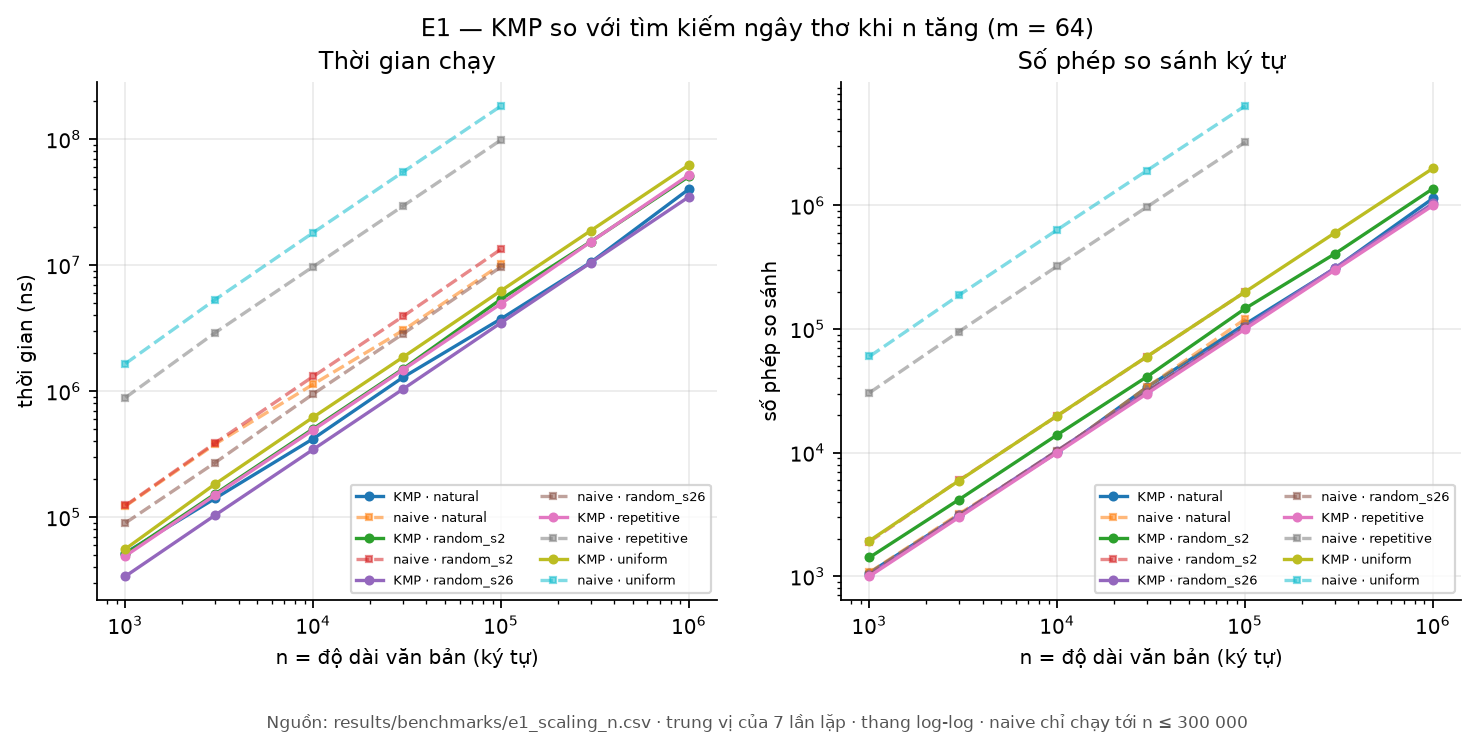
\includegraphics[width=0.94\textwidth,height=0.42\textheight,keepaspectratio]{figures/generated/20b9cab45b828e27cd38dce8b3e7fd22b1856176.png}
\caption{Thời gian chạy và số phép so sánh khi n tăng, thang log-log. Nguồn: results/benchmarks/e1\_scaling\_n.csv, trung vị của 7 lần lặp}
\end{figure}

\begin{figure}[htbp]
\centering
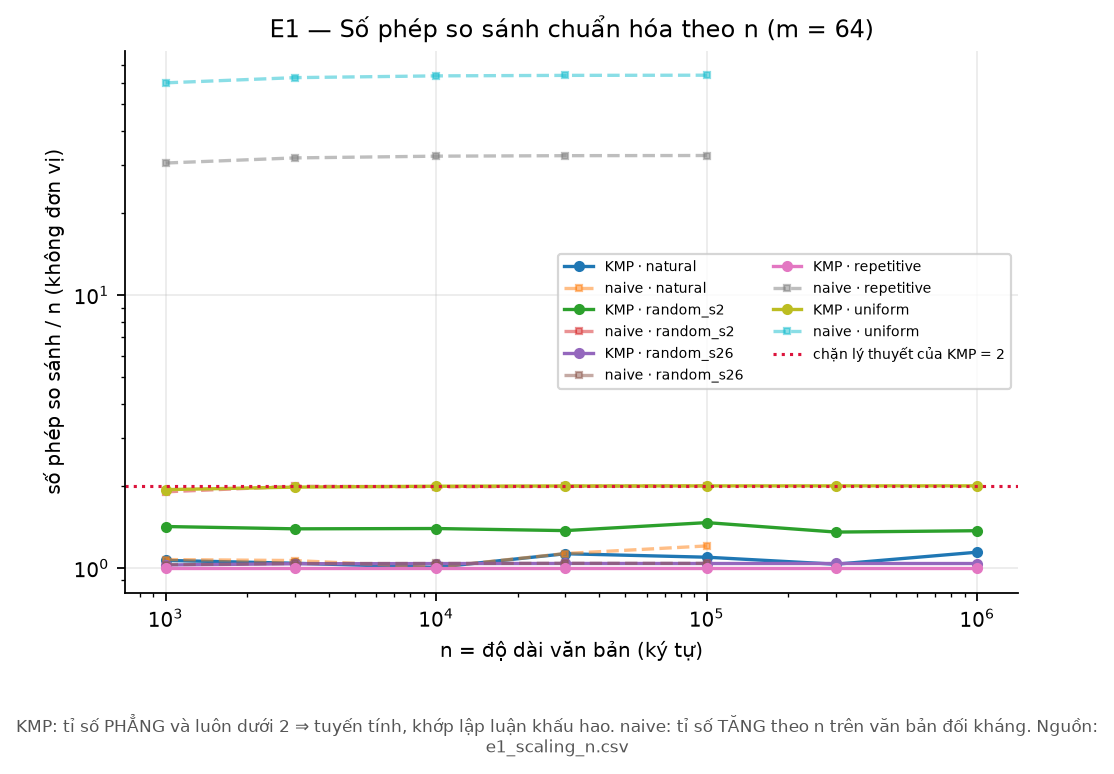
\includegraphics[width=0.94\textwidth,height=0.42\textheight,keepaspectratio]{figures/generated/cd32e43c2503a31ba73e7e8602475fc6cfb0ac8e.png}
\caption{Số phép so sánh chuẩn hóa theo n. Đường KMP nằm phẳng và luôn dưới ngưỡng 2, khớp với lập luận khấu hao ở Định lý 4.1}
\end{figure}

Ba kết luận rút ra từ số liệu này. Thứ nhất, KMP tuyến tính: cột cmp/n
giữ nguyên độ lớn qua ba bậc của n với mọi đặc tính văn bản, không có
dấu hiệu tăng dần. Thứ hai, chặn 2n của Định lý 4.1 là chặt. Trên đầu
vào đối kháng uniform, tỉ số đo được là 1,9999, sát cận trên tới bốn chữ
số thập phân và chưa bao giờ vượt qua. Đây là kiểm chứng định lượng
chính xác nhất trong toàn bộ báo cáo. Thứ ba, thuật toán naive tệ đúng
như dự đoán: trên uniform, tỉ số cmp/n của nó xấp xỉ 64, đúng bằng m,
khớp với chặn O(n·m).

Có một điểm tôi muốn nêu rõ thay vì chỉ trình bày các con số đẹp. Trên
văn bản natural và random\_s26, KMP và naive gần như ngang nhau, tỉ số
chỉ từ 1,0 đến 1,1. Nguyên nhân là với alphabet lớn, xác suất khớp một
phần rất thấp, nên naive hầu như chỉ so sánh một ký tự ở mỗi vị trí rồi
thất bại ngay; nói cách khác nó đã gần tuyến tính trên loại dữ liệu này.
Lợi thế của KMP chỉ bộc lộ khi dữ liệu có cấu trúc lặp. Nếu chỉ trình
bày cột uniform rồi kết luận KMP nhanh hơn naive 32 lần thì đó là phóng
đại.

\section{Thí nghiệm E2 --- ảnh hưởng của độ dài mẫu}
\label{sec:6-5}

Thí nghiệm này cố định n = 30 000 và cho m chạy từ 1 tới 1 024, tức biến
thiên hơn một nghìn lần.

\begin{center}
\captionof{table}{Kết quả thí nghiệm E2 (n = 30 000)}
\end{center}

{\footnotesize\singlespacing
\begin{longtable}[]{@{}
  >{\raggedright\arraybackslash}p{(\linewidth - 10\tabcolsep) * \real{0.0975}}
  >{\centering\arraybackslash}p{(\linewidth - 10\tabcolsep) * \real{0.2145}}
  >{\centering\arraybackslash}p{(\linewidth - 10\tabcolsep) * \real{0.2145}}
  >{\centering\arraybackslash}p{(\linewidth - 10\tabcolsep) * \real{0.1170}}
  >{\centering\arraybackslash}p{(\linewidth - 10\tabcolsep) * \real{0.1949}}
  >{\centering\arraybackslash}p{(\linewidth - 10\tabcolsep) * \real{0.1364}}@{}}
\toprule\noalign{}
\begin{minipage}[b]{\linewidth}\raggedright
m
\end{minipage} & \begin{minipage}[b]{\linewidth}\centering
KMP cmp/n (uniform)
\end{minipage} & \begin{minipage}[b]{\linewidth}\centering
naive cmp/n (uniform)
\end{minipage} & \begin{minipage}[b]{\linewidth}\centering
Tỉ số
\end{minipage} & \begin{minipage}[b]{\linewidth}\centering
KMP cmp/n (natural)
\end{minipage} & \begin{minipage}[b]{\linewidth}\centering
LPS cmp/m
\end{minipage} \\
\midrule\noalign{}
\endhead
\bottomrule\noalign{}
\endlastfoot
1 & 1,000 & 1,000 & 1,0 & 1,000 & 0,00 \\
4 & 1,9999 & 3,9996 & 2,0 & 1,011 & 1,25 \\
16 & 1,9995 & 15,992 & 8,0 & 1,011 & 1,81 \\
64 & 1,9979 & 63,866 & 32,0 & 1,011 & 1,95 \\
256 & 1,9915 & 253,82 & 127,5 & 1,011 & 1,99 \\
1 024 & 1,9659 & --- & --- & 1,010 & 1,997 \\
\end{longtable}
}

\begin{figure}[htbp]
\centering
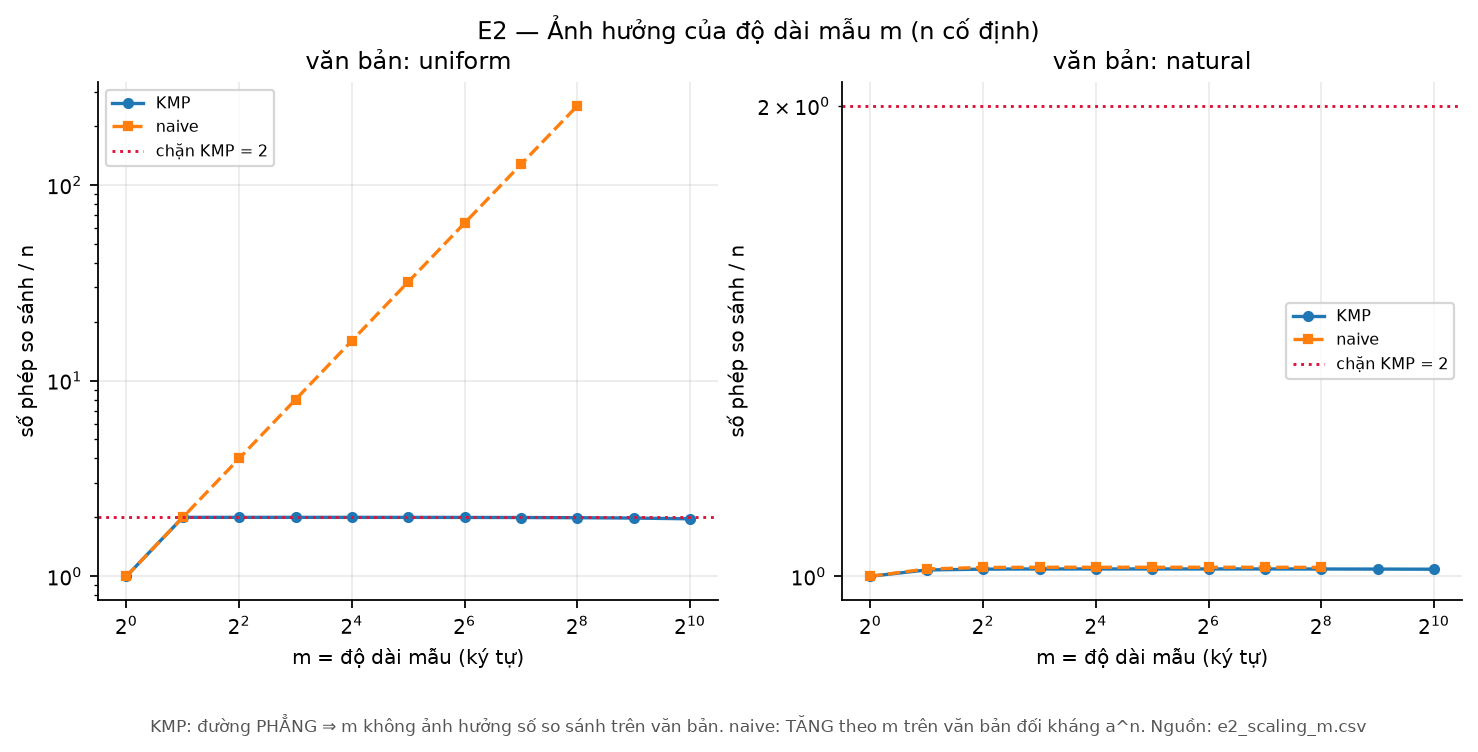
\includegraphics[width=0.94\textwidth,height=0.42\textheight,keepaspectratio]{figures/generated/3fd397c18fa4ddee2a57800acfe209f2f6999e24.png}
\caption{Ảnh hưởng của độ dài mẫu m. Đường KMP nằm ngang, đường naive tăng tuyến tính theo m trên văn bản đối kháng}
\end{figure}

Kết quả xác nhận ba điều. Độ dài mẫu không ảnh hưởng tới số phép so sánh
của KMP trên văn bản: cột KMP giữ nguyên ở khoảng 2,0 với uniform và
1,01 với natural khi m biến thiên 1 024 lần, đúng như Định lý 4.1 phát
biểu rằng chặn là 2n chứ không phải hàm của m. Chặn 2m cho BUILD\_LPS
cũng chặt, tỉ số LPS cmp/m tiến tới 1,997 khi m tăng; với m nhỏ tỉ số
thấp hơn vì chặn mang tính tiệm cận. Còn naive thì tăng tuyến tính theo
m, tỉ số tăng tốc gấp đôi mỗi khi m gấp đôi.

Ở đây có một chi tiết về phương pháp đo đáng ghi lại. Lần chạy đầu tiên
cho cột LPS cmp bằng 0 ở mọi hàng. Nguyên nhân là lớp KMPMatcher tính
prefix function ngay trong hàm khởi tạo để lưu lại dùng nhiều lần, nên
bộ đếm truyền vào phương thức tìm kiếm không bao giờ ghi nhận chi phí
đó. Tôi phải sửa script để đo BUILD\_LPS riêng. Bài học rút ra là một số
0 im lặng rất dễ bị đọc nhầm thành ``chi phí không đáng kể'' trong khi
thực chất là ``phép đo đặt sai chỗ''.

\section{Thí nghiệm E3 --- Trie so với duyệt tuyến tính}
\label{sec:6-6}

\begin{center}
\captionof{table}{Kết quả thí nghiệm E3 với k = 10}
\end{center}

{\footnotesize\singlespacing
\begin{longtable}[]{@{}
  >{\raggedright\arraybackslash}p{(\linewidth - 16\tabcolsep) * \real{0.1422}}
  >{\centering\arraybackslash}p{(\linewidth - 16\tabcolsep) * \real{0.0978}}
  >{\centering\arraybackslash}p{(\linewidth - 16\tabcolsep) * \real{0.1067}}
  >{\centering\arraybackslash}p{(\linewidth - 16\tabcolsep) * \real{0.1067}}
  >{\centering\arraybackslash}p{(\linewidth - 16\tabcolsep) * \real{0.0978}}
  >{\centering\arraybackslash}p{(\linewidth - 16\tabcolsep) * \real{0.1334}}
  >{\centering\arraybackslash}p{(\linewidth - 16\tabcolsep) * \real{0.0978}}
  >{\centering\arraybackslash}p{(\linewidth - 16\tabcolsep) * \real{0.1067}}
  >{\centering\arraybackslash}p{(\linewidth - 16\tabcolsep) * \real{0.0888}}@{}}
\toprule\noalign{}
\begin{minipage}[b]{\linewidth}\raggedright
Từ điển
\end{minipage} & \begin{minipage}[b]{\linewidth}\centering
N
\end{minipage} & \begin{minipage}[b]{\linewidth}\centering
Số nút
\end{minipage} & \begin{minipage}[b]{\linewidth}\centering
nút/ký tự
\end{minipage} & \begin{minipage}[b]{\linewidth}\centering
Trie (µs)
\end{minipage} & \begin{minipage}[b]{\linewidth}\centering
Tuyến tính (µs)
\end{minipage} & \begin{minipage}[b]{\linewidth}\centering
Tăng tốc
\end{minipage} & \begin{minipage}[b]{\linewidth}\centering
search (nút)
\end{minipage} & \begin{minipage}[b]{\linewidth}\centering
byte/từ
\end{minipage} \\
\midrule\noalign{}
\endhead
\bottomrule\noalign{}
\endlastfoot
synthetic & 1 000 & 3 490 & 0,547 & 14,4 & 19,3 & 1,3 & 6 & 734 \\
synthetic & 20 000 & 61 628 & 0,419 & 13,0 & 359,3 & 27,7 & 7 & 636 \\
synthetic & 100 000 & 233 678 & 0,311 & 7,1 & 1 831,6 & 258,6 & 10 &
471 \\
synthetic & 500 000 & 1 075 468 & 0,260 & 8,6 & 9 160,8 & 1 062,1 & 10 &
445 \\
uniform & 1 000 & 6 527 & 0,816 & 8,6 & 38,5 & 4,5 & 8 & 1 442 \\
uniform & 500 000 & 2 311 514 & 0,578 & 17,0 & 9 662,0 & 568,4 & 8 & 1
001 \\
\end{longtable}
}

\begin{figure}[htbp]
\centering
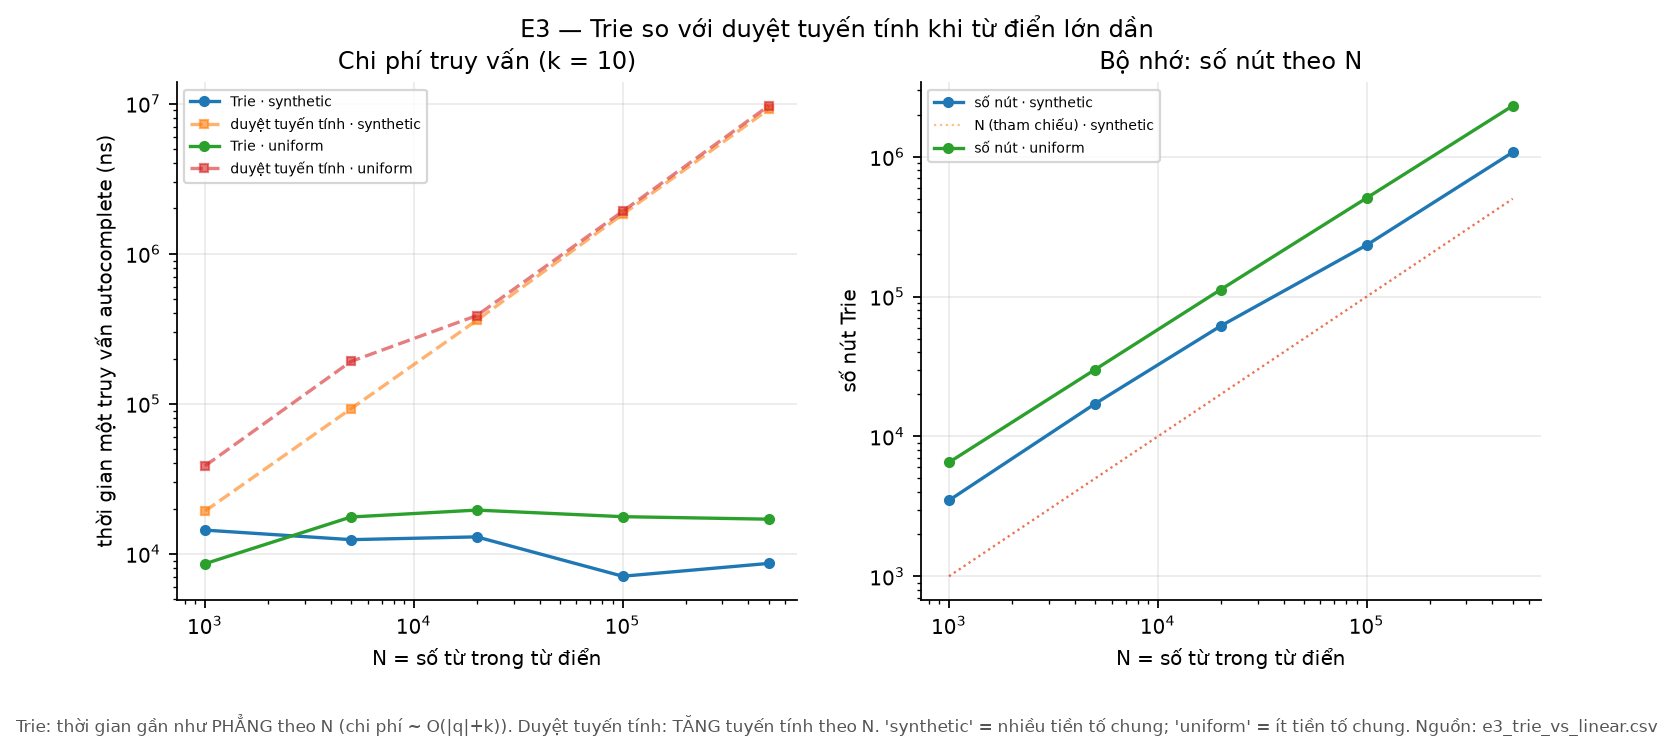
\includegraphics[width=0.94\textwidth,height=0.42\textheight,keepaspectratio]{figures/generated/1030b0be95995c1442eead6599906c0c49250a33.png}
\caption{Trie so với duyệt tuyến tính khi từ điển lớn dần. Bên trái là thời gian một truy vấn autocomplete, bên phải là số nút của cây}
\end{figure}

Chi phí truy vấn Trie không phụ thuộc trực tiếp N: với dữ liệu
synthetic, thời gian nằm trong khoảng 7 đến 14 micro-giây khi N tăng 500
lần. Bằng chứng sạch hơn là exact search chỉ duyệt 6 đến 10 nút, đúng
bằng độ dài từ truy vấn. Ngược lại baseline quét danh sách tăng từ 19
micro-giây lên 9 161 micro-giây; tỉ số đạt 1 062 lần tại N = 500 000.
Đây là số đo của đúng cài đặt, dữ liệu và môi trường đã nêu, không phải
hằng số phổ quát.

Về bộ nhớ, tỉ số nút trên ký tự của synthetic giảm từ 0,547 xuống 0,260
khi N tăng, cho thấy mức chia sẻ tiền tố tăng theo quy mô. Với uniform,
tỉ số tại 500 000 từ vẫn cao hơn, 0,578, và byte trên từ lớn hơn khoảng
2,25 lần. Lợi ích của Trie vì thế phụ thuộc đặc tính dữ liệu chứ không
phải thuộc tính vô điều kiện.

\section{Thí nghiệm E4 --- early stop và trade-off lưu cạnh}
\label{sec:6-7}

\emph{\textbf{6.7.1 Hiệu lực của early stop}}

Thí nghiệm chạy trên từ điển 20 000 từ với một tiền tố dài một ký tự,
tiền tố này có tới 2 513 từ khớp.

\begin{center}
\captionof{table}{Hiệu lực early stop theo k (cây con chứa 2 513 từ)}
\end{center}

{\footnotesize\singlespacing
\begin{longtable}[]{@{}
  >{\raggedright\arraybackslash}p{(\linewidth - 10\tabcolsep) * \real{0.1125}}
  >{\centering\arraybackslash}p{(\linewidth - 10\tabcolsep) * \real{0.1500}}
  >{\centering\arraybackslash}p{(\linewidth - 10\tabcolsep) * \real{0.1687}}
  >{\centering\arraybackslash}p{(\linewidth - 10\tabcolsep) * \real{0.1874}}
  >{\centering\arraybackslash}p{(\linewidth - 10\tabcolsep) * \real{0.1687}}
  >{\centering\arraybackslash}p{(\linewidth - 10\tabcolsep) * \real{0.1874}}@{}}
\toprule\noalign{}
\begin{minipage}[b]{\linewidth}\raggedright
k
\end{minipage} & \begin{minipage}[b]{\linewidth}\centering
Trả về
\end{minipage} & \begin{minipage}[b]{\linewidth}\centering
truncated
\end{minipage} & \begin{minipage}[b]{\linewidth}\centering
Số nút duyệt
\end{minipage} & \begin{minipage}[b]{\linewidth}\centering
Nút/kết quả
\end{minipage} & \begin{minipage}[b]{\linewidth}\centering
Thời gian (µs)
\end{minipage} \\
\midrule\noalign{}
\endhead
\bottomrule\noalign{}
\endlastfoot
1 & 1 & True & 6 & 6,00 & 2,0 \\
10 & 10 & True & 27 & 2,70 & 9,1 \\
100 & 100 & True & 312 & 3,12 & 99,9 \\
1 000 & 1 000 & True & 3 003 & 3,00 & 978 \\
2 513 & 2 513 & False & 7 596 & 3,02 & 2 472 \\
\end{longtable}
}

\begin{figure}[H]
\centering
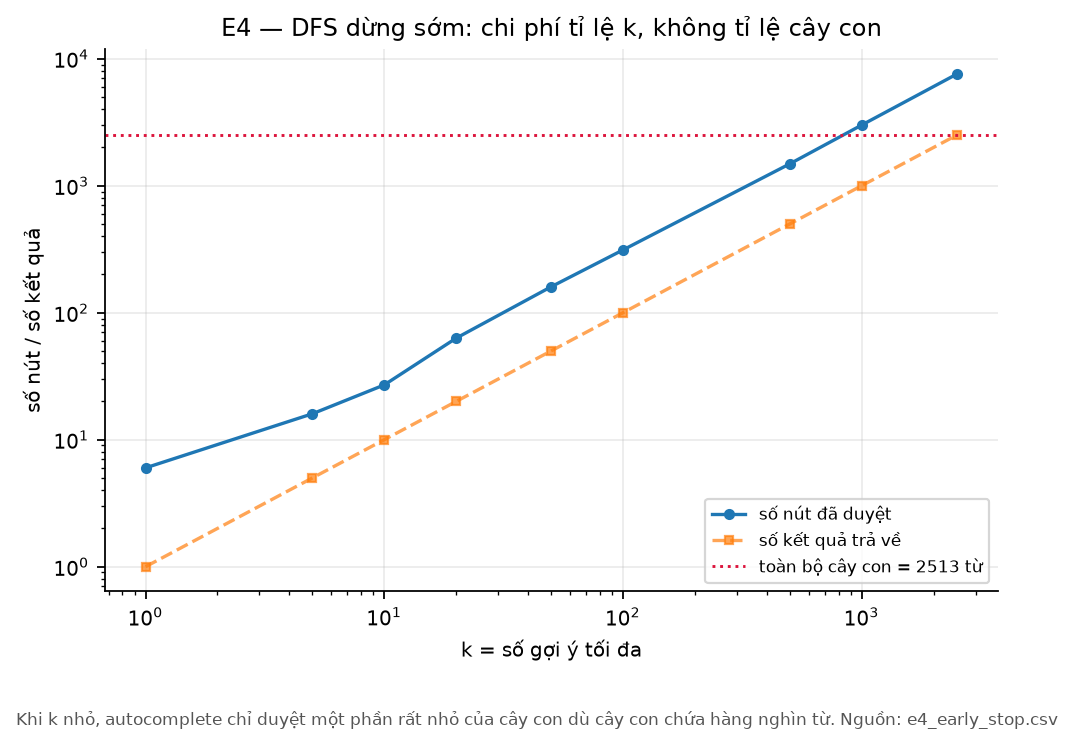
\includegraphics[width=0.94\textwidth,height=0.42\textheight,keepaspectratio]{figures/generated/d0cd0559d67a5aa17231cf53ede12b3d27fd5ac8.png}
\caption{Số nút duyệt tỉ lệ với k chứ không tỉ lệ với kích thước cây con}
\end{figure}

Với k bằng 1, thao tác autocomplete chỉ duyệt 6 nút thay vì 7 596, tức
khoảng tám phần vạn của cây con. Cột nút trên kết quả giữ ổn định quanh
giá trị 3,0, cho thấy chi phí tỉ lệ với k chứ không tỉ lệ với kích thước
cây con. Đây đúng là hành vi mà một ô tìm kiếm cần: người dùng chỉ nhìn
tám tới mười gợi ý, nên chi phí phải theo con số đó chứ không theo tổng
số từ khớp.

\emph{\textbf{6.7.2 Trade-off giữa hash map và mảng}}

\begin{center}
\captionof{table}{Trade-off bộ nhớ giữa hai cách lưu cạnh, \textbar Σ′\textbar{} = 26}
\end{center}

{\footnotesize\singlespacing
\begin{longtable}[]{@{}
  >{\raggedright\arraybackslash}p{(\linewidth - 10\tabcolsep) * \real{0.1365}}
  >{\centering\arraybackslash}p{(\linewidth - 10\tabcolsep) * \real{0.1559}}
  >{\centering\arraybackslash}p{(\linewidth - 10\tabcolsep) * \real{0.2145}}
  >{\centering\arraybackslash}p{(\linewidth - 10\tabcolsep) * \real{0.1755}}
  >{\centering\arraybackslash}p{(\linewidth - 10\tabcolsep) * \real{0.1559}}
  >{\centering\arraybackslash}p{(\linewidth - 10\tabcolsep) * \real{0.1365}}@{}}
\toprule\noalign{}
\begin{minipage}[b]{\linewidth}\raggedright
N
\end{minipage} & \begin{minipage}[b]{\linewidth}\centering
Số nút
\end{minipage} & \begin{minipage}[b]{\linewidth}\centering
Ô mảng cấp phát
\end{minipage} & \begin{minipage}[b]{\linewidth}\centering
hash map (KB)
\end{minipage} & \begin{minipage}[b]{\linewidth}\centering
mảng (KB)
\end{minipage} & \begin{minipage}[b]{\linewidth}\centering
Tỉ số
\end{minipage} \\
\midrule\noalign{}
\endhead
\bottomrule\noalign{}
\endlastfoot
1 000 & 3 074 & 79 924 & 630 & 964 & 1,53 \\
5 000 & 15 486 & 402 636 & 3 231 & 4 870 & 1,51 \\
20 000 & 61 628 & 1 602 328 & 12 898 & 19 397 & 1,50 \\
\end{longtable}
}

\begin{figure}[htbp]
\centering
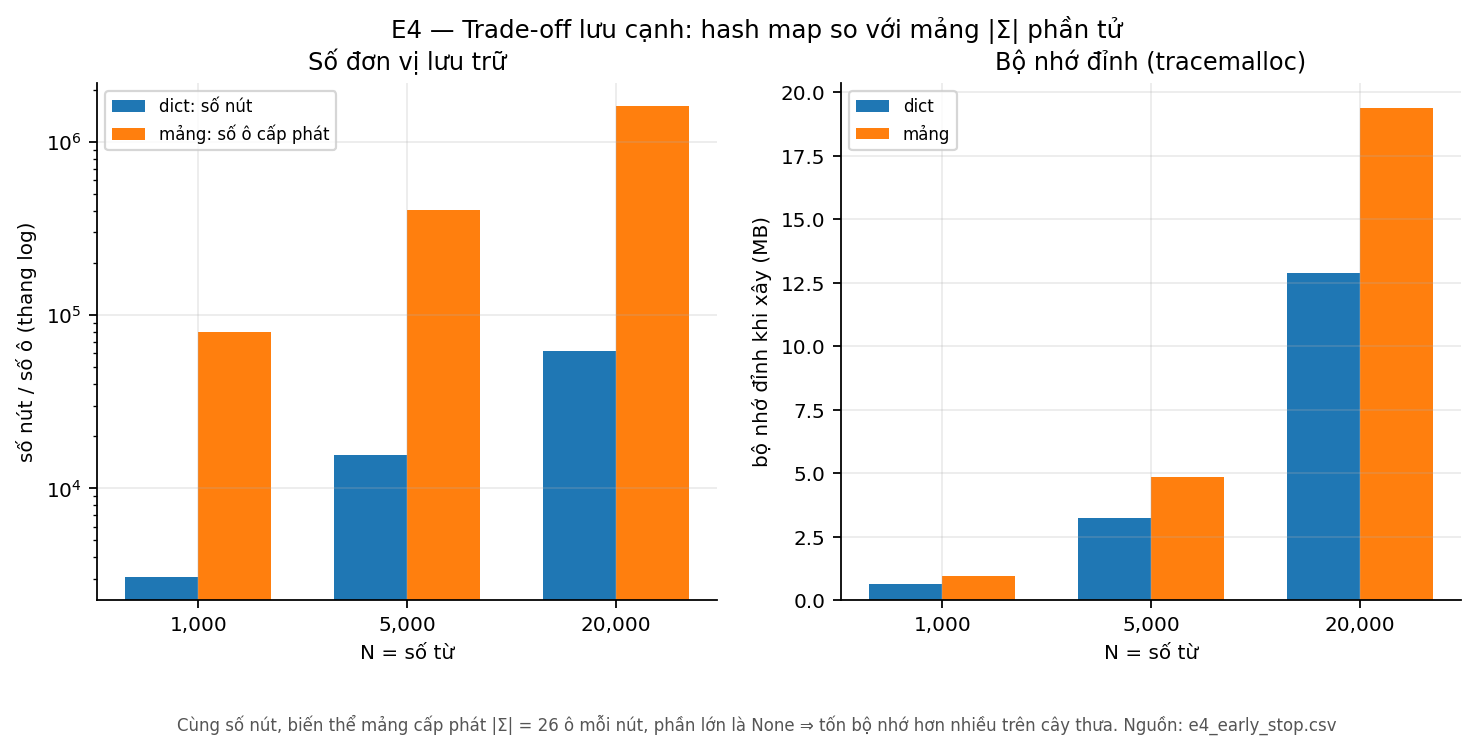
\includegraphics[width=0.94\textwidth,height=0.42\textheight,keepaspectratio]{../../results/figures/fig6_storage_tradeoff.png}
\caption{Số đơn vị lưu trữ và bộ nhớ đỉnh của hai biến thể. Chênh lệch về số ô cấp phát lớn hơn nhiều so với chênh lệch bộ nhớ thực đo}
\end{figure}

Kết quả này đi ngược trực giác và tôi giữ nguyên nó. Biến thể mảng cấp
phát nhiều hơn 26 lần số ô, cụ thể 1,6 triệu ô so với 61 628 nút, nhưng
bộ nhớ đỉnh chỉ cao hơn 1,50--1,53 lần. Nguyên nhân nằm ở cách CPython tổ chức
bộ nhớ: một ô trong danh sách chứa giá trị None chỉ tốn 8 byte con trỏ,
trong khi mỗi đối tượng từ điển mang theo phần dư cố định khá lớn gồm
bảng băm và phần đầu đối tượng. Nói cách khác, ở mức
\textbar Σ′\textbar{} bằng 26, chi phí của 26 con trỏ rỗng chưa vượt
được chi phí của một từ điển rỗng.

Hệ quả cần phát biểu cẩn thận: kết luận rằng biến thể mảng tốn bộ nhớ
hơn là kết luận tiệm cận theo \textbar Σ′\textbar, không phải kết luận
đúng với mọi \textbar Σ′\textbar. Với alphabet tiếng Việt gồm 105 ký tự,
tỉ số nhiều khả năng sẽ đảo chiều rõ rệt, nhưng tôi chưa đo trực tiếp
nên đây vẫn là ngoại suy. Lý do tôi vẫn chọn hash map không chỉ nằm ở tỉ số
1,50--1,53 lần này mà còn ở chỗ biến thể mảng buộc phải biết
\textbar Σ′\textbar{} tại thời điểm tạo mỗi nút, điều gây bất tiện khi
hệ thống cần hỗ trợ nhiều alphabet khác nhau.

\section{Thí nghiệm E5 --- Aho--Corasick so với KMP lặp lại}
\label{sec:6-8}

\begin{center}
\captionof{table}{Kết quả thí nghiệm E5 trên văn bản n = 100 000}
\end{center}

{\footnotesize\singlespacing
\begin{longtable}[]{@{}
  >{\raggedright\arraybackslash}p{(\linewidth - 10\tabcolsep) * \real{0.1351}}
  >{\centering\arraybackslash}p{(\linewidth - 10\tabcolsep) * \real{0.1447}}
  >{\centering\arraybackslash}p{(\linewidth - 10\tabcolsep) * \real{0.1738}}
  >{\centering\arraybackslash}p{(\linewidth - 10\tabcolsep) * \real{0.2123}}
  >{\centering\arraybackslash}p{(\linewidth - 10\tabcolsep) * \real{0.1544}}
  >{\centering\arraybackslash}p{(\linewidth - 10\tabcolsep) * \real{0.1544}}@{}}
\toprule\noalign{}
\begin{minipage}[b]{\linewidth}\raggedright
Số mẫu
\end{minipage} & \begin{minipage}[b]{\linewidth}\centering
Số nút AC
\end{minipage} & \begin{minipage}[b]{\linewidth}\centering
AC (so sánh)
\end{minipage} & \begin{minipage}[b]{\linewidth}\centering
KMP lặp (so sánh)
\end{minipage} & \begin{minipage}[b]{\linewidth}\centering
Tỉ số so sánh
\end{minipage} & \begin{minipage}[b]{\linewidth}\centering
Tỉ số thời gian
\end{minipage} \\
\midrule\noalign{}
\endhead
\bottomrule\noalign{}
\endlastfoot
1 & 7 & 109 539 & 108 737 & 0,99 & 0,66 \\
2 & 14 & 110 561 & 209 758 & 1,90 & 1,16 \\
5 & 25 & 132 758 & 532 318 & 4,01 & 2,61 \\
10 & 63 & 144 341 & 1 057 779 & 7,33 & 4,96 \\
25 & 133 & 150 807 & 2 612 143 & 17,3 & 10,95 \\
50 & 275 & 149 087 & 5 220 240 & 35,0 & 20,62 \\
100 & 499 & 148 241 & 10 440 185 & 70,4 & 39,72 \\
\end{longtable}
}

\begin{figure}[htbp]
\centering
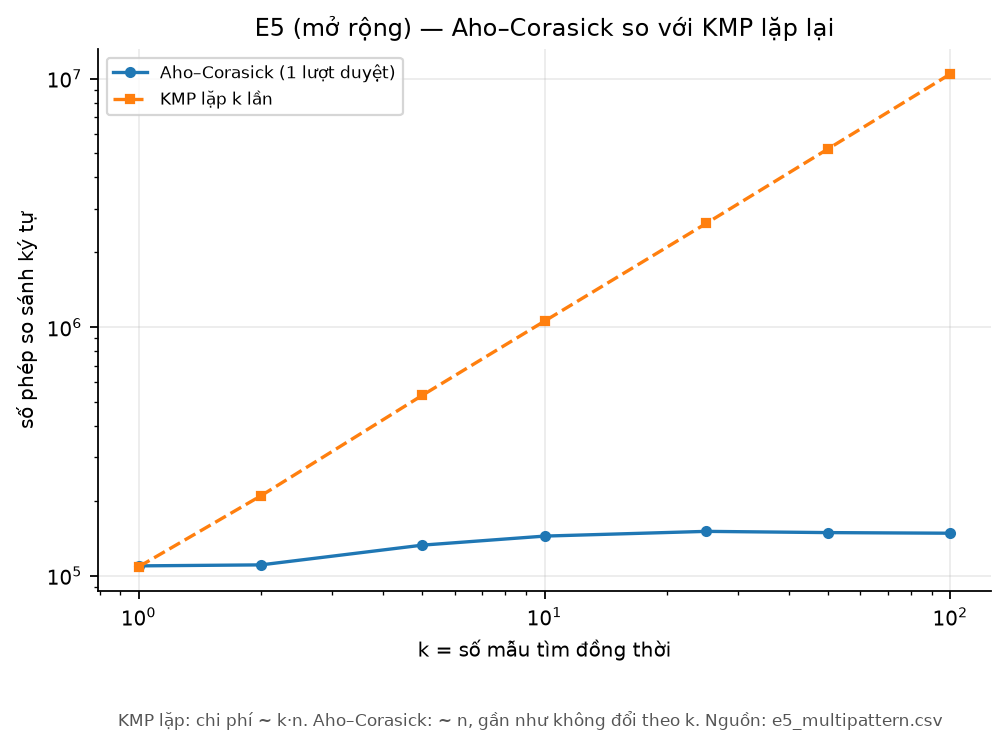
\includegraphics[width=0.94\textwidth,height=0.42\textheight,keepaspectratio]{figures/generated/7256f92caee80417225f2d1803f59b9a7be96ee1.png}
\caption{Aho--Corasick so với KMP lặp nhiều lần. Chi phí của Aho--Corasick gần như không đổi khi số mẫu tăng}
\end{figure}

Số phép so sánh của Aho--Corasick gần như đứng yên, từ 109 539 lên 148
241 khi số mẫu tăng gấp trăm lần, trong khi KMP lặp tăng tuyến tính theo
số mẫu. Điều này khớp chính xác với độ phức tạp O(n +
Σ\textbar Pᵢ\textbar{} + số khớp) so với O(k·n + Σ\textbar Pᵢ\textbar).

Dòng đầu tiên cho thấy với đúng một mẫu, Aho--Corasick chậm hơn KMP, tỉ
số thời gian chỉ 0,66. Mở rộng không tốt hơn vô điều kiện mà chỉ bắt đầu
có lợi từ hai mẫu trở lên; đối tượng nút và hash map có hằng số lớn hơn
truy cập mảng π.

\section{Đối chiếu tổng hợp giữa lý thuyết và số liệu}
\label{sec:6-9}

\begin{center}
\captionof{table}{Đối chiếu chín khẳng định lý thuyết với số liệu đo}
\end{center}

{\footnotesize\singlespacing
\begin{longtable}[]{@{}
  >{\raggedright\arraybackslash}p{(\linewidth - 6\tabcolsep) * \real{0.2918}}
  >{\raggedright\arraybackslash}p{(\linewidth - 6\tabcolsep) * \real{0.2334}}
  >{\raggedright\arraybackslash}p{(\linewidth - 6\tabcolsep) * \real{0.3113}}
  >{\raggedright\arraybackslash}p{(\linewidth - 6\tabcolsep) * \real{0.1362}}@{}}
\toprule\noalign{}
\begin{minipage}[b]{\linewidth}\raggedright
Khẳng định
\end{minipage} & \begin{minipage}[b]{\linewidth}\raggedright
Cách kiểm chứng
\end{minipage} & \begin{minipage}[b]{\linewidth}\raggedright
Kết quả đo
\end{minipage} & \begin{minipage}[b]{\linewidth}\raggedright
Khớp
\end{minipage} \\
\midrule\noalign{}
\endhead
\bottomrule\noalign{}
\endlastfoot
KMP: số so sánh ≤ 2n (Định lý 4.1) & E1, mọi đặc tính, n tới 10\textsuperscript{6} & tối
đa 1,9999·n & có \\
BUILD\_LPS: số so sánh ≤ 2m & E2, m tới 1 024 & tối đa 1,997·m & có \\
KMP không phụ thuộc m & E2, m biến thiên 1 024 lần & cmp/n giữ nguyên &
có \\
naive là Θ(n·m) & E1 và E2 & cmp/n xấp xỉ m & có \\
Trie search là Θ(L), độc lập N & E3, N biến thiên 500 lần & 6--10 nút,
bằng độ dài từ & có \\
Trie tiết kiệm nhờ chia sẻ tiền tố & E3, cột nút/ký tự & 0,26 tới 0,82,
đều dưới 1 & có \\
autocomplete early stop giảm V & E4(a) & số nút xấp xỉ 3k, độc lập cây
con & có \\
mảng tốn bộ nhớ hơn hash map & E4(b) & 1,50--1,53 lần ở
\textbar Σ′\textbar{} = 26 & một phần \\
Aho--Corasick O(n) theo số mẫu & E5, tới 100 mẫu & số so sánh gần như
không đổi & có \\
\end{longtable}
}

Tám trên chín khẳng định được số liệu xác nhận đầy đủ. Khẳng định thứ
tám đúng về hướng nhưng sai đáng kể về độ lớn, và nguyên nhân đã được
phân tích ở Mục 6.7.2: đó là hệ quả của chi tiết cài đặt trong CPython
chứ không phải sai sót của lý thuyết. Tôi chọn giữ nguyên kết quả này
trong báo cáo kèm phần giải thích, thay vì lược bỏ nó để bảng nhìn cho
gọn.

\chapter{ỨNG DỤNG, GIỚI HẠN\\VÀ HƯỚNG MỞ RỘNG}
\label{ch:7}

\section{Hai giao diện của hệ thống}
\label{sec:7-1}

CLI hỗ trợ tìm KMP, gợi ý Trie, xem prefix function, chạy
Aho--Corasick và in số đếm thao tác. Giao diện web chạy cục bộ bằng
thư viện chuẩn: gợi ý cập nhật khi gõ, kết quả được tô sáng, còn prefix
function và dãy border hiện theo thời gian thực. Hai giao diện dùng
chung tầng dịch vụ nên cũng là phép kiểm tra tích hợp.

\section{Giới hạn và các trường hợp không nên dùng}
\label{sec:7-2}

\begin{center}
\captionof{table}{Giới hạn chính và hướng thay thế}
\end{center}

{\footnotesize\singlespacing
\begin{longtable}[]{@{}
  >{\raggedright\arraybackslash}p{(\linewidth - 2\tabcolsep) * \real{0.46}}
  >{\raggedright\arraybackslash}p{(\linewidth - 2\tabcolsep) * \real{0.50}}@{}}
\toprule\noalign{}
\begin{minipage}[b]{\linewidth}\raggedright
Tình huống
\end{minipage} & \begin{minipage}[b]{\linewidth}\raggedright
Nên dùng gì
\end{minipage} \\
\midrule\noalign{}
\endhead
\bottomrule\noalign{}
\endlastfoot
Nhiều truy vấn trên cùng văn bản tĩnh & suffix array
\cite{manber1993} hoặc suffix tree \cite{ukkonen1995} \\
Nhiều mẫu đồng thời & Aho--Corasick \cite{aho1975}, đã cài ở Mục 7.3 \\
Tìm mờ hoặc chịu lỗi chính tả & Trie kết hợp khoảng cách chỉnh sửa
\cite{navarro2001} \\
Từ điển rất lớn, alphabet rộng & PATRICIA \cite{morrison1968},
burst trie \cite{heinz2002} hoặc HAT-trie \cite{askitis2007} \\
Văn bản vượt RAM hoặc cần xóa từ & KMP streaming; bổ sung delete bảo
toàn I3 và I4 \\
\end{longtable}
}

Hệ thống phù hợp với từ điển tĩnh, văn bản vừa RAM và phép khớp chính
xác. Tôi không khẳng định mã KMP Python nhanh hơn \texttt{str.find};
hàm chuẩn viết bằng C và dùng thuật toán two-way \cite{crochemore1991}.
Giá trị của module là trả mọi vị trí overlapping với chặn 2n chứng minh
được, không phải tốc độ tuyệt đối.

\section{Phần mở rộng đã cài: Aho--Corasick}
\label{sec:7-3}

Aho--Corasick \cite{aho1975} đặt failure link lên Trie của nhiều mẫu;
đó là dạng tổng quát của prefix function. Link được dựng bằng BFS, còn
output link nén chuỗi failure để chi phí liệt kê tỉ lệ số khớp. Một
property test kiểm chứng: với đúng một mẫu, độ sâu failure link trùng
prefix function trên bảy mẫu cố định và một nghìn mẫu ngẫu nhiên.

\section{Hướng phát triển}
\label{sec:7-4}

Ba hướng ưu tiên là compressed trie để giảm số nút, lưu top-k tại mỗi
nút để xếp hạng mà vẫn dừng sớm, và tìm gần đúng chịu lỗi chính tả. Với
văn bản lớn, có thể thêm streaming hoặc tiền xử lý suffix array; mọi
ước lượng chưa đo đều được giữ ở trạng thái giả thuyết.

\chapter{KẾT LUẬN}
\label{ch:8}

\section{Kết quả đạt được}
\label{sec:8-1}

Sản phẩm gồm hai module độc lập KMP--Trie, prefix function công khai,
năm alphabet, Aho--Corasick và hai giao diện demo; mã xử lý đầy đủ đầu
vào biên, ký tự không hợp lệ và khớp overlapping. Báo cáo chứng minh
tính đúng bằng border, bất biến vòng lặp và lập luận khấu hao, trong đó
hai chặn 2n và 2m được kiểm chứng tới bốn chữ số thập phân.

Toàn bộ 276 test và 10 doctest đều pass; ba baseline độc lập, sáu
property test và seed cố định hỗ trợ kiểm tra chéo. Năm nhóm thí nghiệm
sinh sáu bảng kết quả, bảy biểu đồ và tệp môi trường; tám trong chín
khẳng định được xác nhận đầy đủ, khẳng định còn lại được xác nhận về
hướng và giải thích bằng chi tiết bộ nhớ CPython.

\section{Những phần chưa hoàn thành}
\label{sec:8-2}

\begin{enumerate}
\item
  Hai baseline có giới hạn công bố trước: E3 giả thiết danh sách đã sắp,
  loại trùng; naive được bỏ qua khi $n\cdot m>8\cdot10^6$. Mọi ô bị bỏ
  đều ghi rõ lý do trong CSV.
\item
  Trie chưa có delete và chưa được nén; trade-off lưu cạnh mới đo với
  $\lvert\Sigma'\rvert=26$, nên kết luận cho alphabet 105 ký tự vẫn là
  hướng thực nghiệm tiếp theo.
\item
  Số liệu thời gian gắn với CPython 3.11 trên macOS arm64, không so sánh
  trực tiếp với C++17; chỉ số đếm thao tác và xu hướng tiệm cận có thể
  chuyển sang ngôn ngữ khác.
\end{enumerate}

\section{Phạm vi đóng góp cá nhân}
\label{sec:8-3}

Trong sản phẩm nộp cá nhân này, Huỳnh Phát Lợi chịu trách nhiệm tích hợp
KMP và Trie thành hai giao diện demo, cài phần mở rộng Aho--Corasick,
thiết kế pipeline dữ liệu--benchmark--biểu đồ có seed và mã băm, kiểm tra
chéo kết quả, và hoàn thiện báo cáo. Phân công của cả nhóm và phần trình
bày tương ứng được công bố ở slide 2 của tệp thuyết trình.

\section{Bài học rút ra từ quá trình thực hiện}
\label{sec:8-4}

Kiểm thử đã phát hiện cả lỗi giả định lẫn lỗi đo: một kỳ vọng sai về dãy
border của ``abaaba'', một doctest nhầm thứ tự từ điển, và bộ đếm chi
phí BUILD\_LPS đặt sai vị trí. Bài học quan trọng nhất là đo số phép so
sánh bên cạnh thời gian: số đếm kiểm chứng trực tiếp chặn lý thuyết và
ít phụ thuộc ngôn ngữ, phần cứng hơn số nano-giây.
